%% 
%% Copyright 2007-2024 Elsevier Ltd
%% 
%% This file is part of the 'Elsarticle Bundle'.
%% ---------------------------------------------
%% 
%% It may be distributed under the conditions of the LaTeX Project Public
%% License, either version 1.3 of this license or (at your option) any
%% later version.  The latest version of this license is in
%%    http://www.latex-project.org/lppl.txt
%% and version 1.3 or later is part of all distributions of LaTeX
%% version 1999/12/01 or later.
%% 
%% The list of all files belonging to the 'Elsarticle Bundle' is
%% given in the file `manifest.txt'.
%% 
%% Template article for Elsevier's document class `elsarticle'
%% with numbered style bibliographic references
%% SP 2008/03/01
%% $Id: elsarticle-template-num.tex 249 2024-04-06 10:51:24Z rishi $
%%
\documentclass[preprint,12pt]{elsarticle}

%% Use the option review to obtain double line spacing
%% \documentclass[authoryear,preprint,review,12pt]{elsarticle}

%% Use the options 1p,twocolumn; 3p; 3p,twocolumn; 5p; or 5p,twocolumn
%% for a journal layout:
%% \documentclass[final,1p,times]{elsarticle}
%% \documentclass[final,1p,times,twocolumn]{elsarticle}
%% \documentclass[final,3p,times]{elsarticle}
%% \documentclass[final,3p,times,twocolumn]{elsarticle}
%% \documentclass[final,5p,times]{elsarticle}
%% \documentclass[final,5p,times,twocolumn]{elsarticle}

%% For including figures, graphicx.sty has been loaded in
%% elsarticle.cls. If you prefer to use the old commands
%% please give \usepackage{epsfig}

%% The amssymb package provides various useful mathematical symbols
\usepackage{amssymb}
%% The amsmath package provides various useful equation environments.
\usepackage{amsmath}
%% The amsthm package provides extended theorem environments
\usepackage{amsthm}

%% The lineno packages adds line numbers. Start line numbering with
%% \begin{linenumbers}, end it with \end{linenumbers}. Or switch it on
%% for the whole article with \linenumbers.
\usepackage{lineno}

\usepackage{graphicx} %Loading the package
\usepackage{subcaption}
\usepackage{hyperref}
\usepackage{xcolor}

\graphicspath{{figures/}} %Setting the graphicspath

\journal{Elsevier}

\begin{document}

\begin{frontmatter}

%% Title, authors and addresses

%% use the tnoteref command within \title for footnotes;
%% use the tnotetext command for theassociated footnote;
%% use the fnref command within \author or \affiliation for footnotes;
%% use the fntext command for theassociated footnote;
%% use the corref command within \author for corresponding author footnotes;
%% use the cortext command for theassociated footnote;
%% use the ead command for the email address,
%% and the form \ead[url] for the home page:
%% \title{Title\tnoteref{label1}}
%% \tnotetext[label1]{}
%% \author{Name\corref{cor1}\fnref{label2}}
%% \ead{email address}
%% \ead[url]{home page}
%% \fntext[label2]{}
%% \cortext[cor1]{}
%% \affiliation{organization={},
%%             addressline={},
%%             city={},
%%             postcode={},
%%             state={},
%%             country={}}
%% \fntext[label3]{}

\title{Analysis of finite-volume advection schemes on cubed-sphere grids and an accurate \textcolor{red}{scheme} for divergent winds}

%% use optional labels to link authors explicitly to addresses:
%% \author[label1,label2]{}
%% \affiliation[label1]{organization={},
%%             addressline={},
%%             city={},
%%             postcode={},
%%             state={},
%%             country={}}
%%
%% \affiliation[label2]{organization={},
%%             addressline={},
%%             city={},
%%             postcode={},
%%             state={},
%%             country={}}

\author[1]{Luan F. Santos\corref{cor1}}
\ead{luan.santos@usp.br}

\author[1]{Pedro S. Peixoto}
\ead{ppeixoto@usp.br}

 \cortext[cor1]{Corresponding author}

%% Author affiliation

\affiliation[1]{organization={Instituto de Matemática e Estatística, Universidade de São Paulo}, 
	addressline={Rua do Matão, 1010},
	postcode={05508-090}, 
	city={São Paulo}, 
	country={Brazil}}




%% Abstract
\begin{abstract}
%% Text of abstract
To be written.
\end{abstract}

%%Graphical abstract
%\begin{graphicalabstract}
%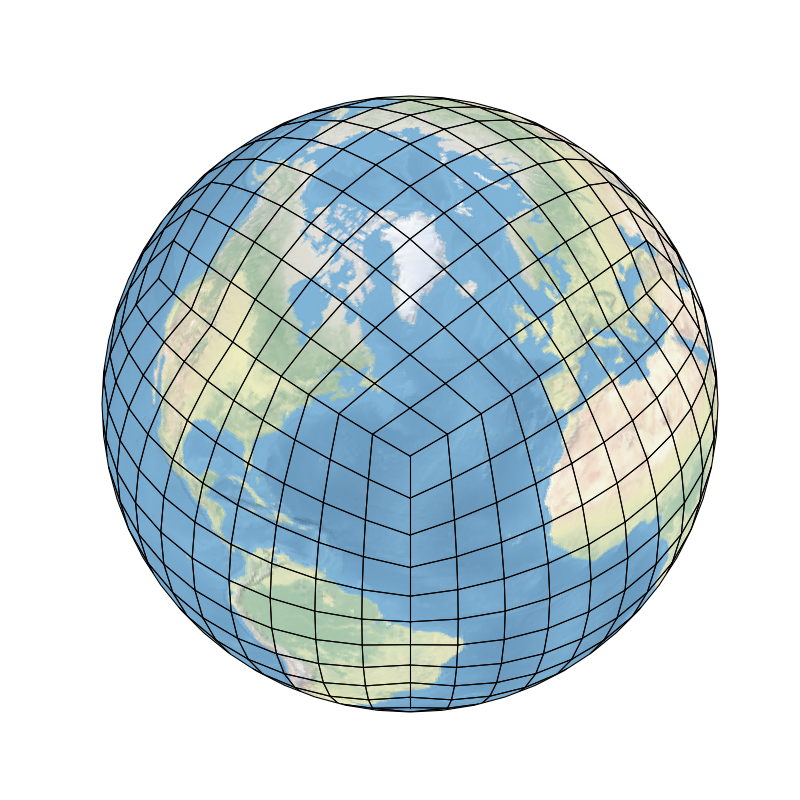
\includegraphics[width=.4\linewidth]{gnomonic_equiangular_cs_10_sphere}
%\end{graphicalabstract}

%%Research highlights
\begin{highlights}
\item To be written.
\item To be written.
\end{highlights}

%% Keywords
\begin{keyword}
Cubed-sphere,
finite-volume,
transport,
advection,
\textcolor{red}{
atmosphere dynamics,
numerical weather prediction,
divergent winds}.
\end{keyword}

\end{frontmatter}
\begin{linenumbers}
%% Add \usepackage{lineno} before \begin{document} and uncomment 
%% following line to enable line numbers
%% \linenumbers

%% main text
%%

\newpage
%%%%%%%%%%%%%%%%%%%%%%%%%%%%%%%%%%%%%%%%%%%%%%%%%%%%%%%%%%%%%%
\section{Introduction}
\label{intro}
The Finite Volume Cubed-Sphere Dynamical Core (FV3), developed by the Geophysical Fluid Dynamics Laboratory (GFDL) and the National Oceanic and Atmospheric Administration (NOAA), 
has been embraced as the dynamical core for several atmospheric models (cf. eg. \cite{zhou:2015,lee:2020, bertrand:2020,harris:2020,martin:2022,zhang:2024}).
In 2019, FV3 attained significant recognition when it was adopted as the new dynamical core for the Global Forecast System the U.S. National Weather Service (NWS), replacing the spectral transform GFS.
Additionally, FV3 is used in the Hurricane Analysis and Forecast System (HAFS) from the NWS for tropical cyclone forecasts \cite{dong:2020}.
 % (\url{https://www.noaa.gov/media-release/noaa-upgrades-us-global-weather-forecast-model}, last
%accessed on April 19th, 2024).


Currently, FV3 solves the non-hydrostatic and compressible Euler equations employing the vertical Lagrangian coordinate approach outlined in \cite{lin:2004}.
This method entails solving the shallow-water equations (SWEs) on designated Lagrangian surfaces. 
Consequently, the SWEs solver assume a pivotal role within the FV3 non-hydrostatic solver.

On the other hand, within FV3, the solution to the SWEs is derived using the method proposed by \cite{lin:1997} extended to the cubed-sphere grid.
This approach takes into account the SWEs in their vector invariant form, along with the C and D-grids introduced by \cite{arakawa:1977}.
A major feature of this scheme is that the computation of fluid pressure, absolute vorticity, and kinetic energy fluxes is carried out using only transport finite-volume fluxes. 

Furthermore, the method of  \cite{lin:1997} involves initially solving the SWEs for a half time-step to acquire C-grid covariant wind components, 
which are then utilized to advance the D-grid covariant wind components for a full time step. 
The C-grid half-step makes use of computationally inexpensive upwind flux operators, while the D-grid incorporates the FV3 transport scheme fluxes proposed by \cite{lin:1996,putman:2007}.
Consequently, this method relies entirely on transport finite-volume fluxes. 
Thus, the transport scheme assumes a critical role in shaping the horizontal dynamics of FV3, beyond its traditional function in the dynamical core, as observed in tracer transport \cite{will:2007}.

The transport scheme employed in FV3 extends the method introduced by \cite{lin:1996} to the cubed-sphere, as proposed by \cite{putman:2007}. 
This approach involves constructing a two-dimensional (2D) scheme by combining the solution of one-dimensional (1D) conservative transport equations using a direction-splitting strategy on each cube face.
The 1D equations are solved using the finite-volume approach of the Piecewise Parabolic Method (PPM) \cite{colella:1984,carpenter:1990}. 
A notable feature of the scheme proposed by \cite{lin:1996} is its elimination of the splitting error under conditions where the initial transported scalar field density is constant and the wind is divergence-free. 
This property is attained through modifications to the inner advection operators employed within the scheme.

The goal of this study is to reassess and suggest enhancements for the current FV3 transport scheme originally developed by \cite{putman:2007}, given its pivotal role in the horizontal dynamics of FV3. 
We demonstrate that the scheme proposed by \cite{putman:2007} assumes constant metric terms during the application of the PPM to each 1D flux integration domain and employs a first-order departure point calculation for the 1D fluxes.
We propose the development of a scheme that incorporates a second-order departure point calculation for the 1D fluxes and eliminates the assumption of constant metric terms. 
While the proposed scheme does not retain the property of splitting error elimination for divergence-free winds and constant scalar fields, it introduces only second-order errors in such scenarios.

The proposed scheme performs slightly better for divergence-free wind simulations of the advection equation on the sphere.
Notably, the proposed scheme achieves second-order accuracy for divergent winds, while the FV3 scheme is only first-order accurate in this scenario.
Furthermore,  the proposed scheme is easy to implement in the current FV3 code and adds only a small extra computational cost.
The extra cost is mainly due to the second-order departure point computation, which requires 1D linear interpolations at each cell edge in both directions of each cubed-sphere panel.

This work is outlined as follows:
in Section \ref{cs-grids}, we present the cubed-sphere grids, revisiting both the equiangular and equi-edge grids, and also discuss the treatment of ghost cells, providing all the tools we shall need during this work.
In Section \ref{adv-2d}, we revisited the FV3 transport scheme on the cubed-sphere and we propose the new scheme.
In Section \ref{num-exp}, we present numerical simulations comparing the proposed scheme with the current FV3 transport scheme. 
Final thoughts are presented in Section \ref{conclusion}.

\newpage
%%%%%%%%%%%%%%%%%%%%%%%%%%%%%%%%%%%%%%%%%%%%%%%%%%%%%%%%%%%%%%
\section{Cubed-sphere grids}
\label{cs-grids}
The goal of this section is to review the concept of cubed-sphere grids, particularly those available in FV3.
To start with, we are going to present the mapping between the cube and the sphere introduced by \cite{sadourny:1972} in section \ref{cs-equidistant}, also known as the equidistant mapping.
Following that, we show that using a change of coordinates, we may use the equidistant mapping to create other mappings from the cube to the sphere.
Namely, section \ref{cs-equiangular} introduces the equiangular mapping introduced by \cite{ronchi:1996}, and section \ref{cs-equiedge} introduces the equi-edge mapping introduced by \cite{chen:2021}. 
In section \ref{cs-grid}, we demonstrate how these mappings are utilized to generate cubed-sphere grids. 
We mainly introduce all the notations and tools that will be needed for the remainder of this work.
Finally, in section \ref{cs-ghost}, we demonstrate how the ghost cells that we will need are generated.

%%%%%%%%%%%%%%%%%%%%%%%%%%%%%%%%%%%%%%%%%%%%%%%%%%%%%%%%%%%%%%
\subsection{Equidistant mapping}
\label{cs-equidistant}
The mapping introduced by \cite{sadourny:1972} between the cube and the sphere divides the sphere into six quadrilaterals, also called panels, and enables the tessellation of the sphere into smaller quadrilaterals for each panel.
This mapping is also called equidistant mapping and generates the equidistant grid.
Given $R>0$, the sphere of radius $R$ 
centered at the origin of  $\mathbb{R}^3$ is denoted as:
\begin{equation}
	\label{s2_r}
	\mathbb{S}^2_R = \{ P = (p_x,p_y,p_z) \in \mathbb{R}^3: p_x^2 + p_y^2 + p_z^2 = R^2\}.
\end{equation}
For the purposes of this work, the Earth radius $R=6.371\times 10^6$ meters is considered.
The equidistant mapping considers a cube centered at the origin with a side length of $\frac{2R}{\sqrt{3}}$ and radially projects the cube faces onto the sphere (Figure \ref{sph-cube-equidist}).

The equidistant mapping is a family of maps ${\Gamma}_{p}: [-1,1] \times [-1,1] \to \mathbb{S}^2_R$, where $p=1, \ldots, 6$, defined as follows:
\begin{align}
	\label{gamma_1}
	{\Gamma}_{1}(X,Y) &= \frac{R}{\sqrt{1 + X^2 + Y^2}}(1, X, Y),\\ 
	\label{gamma_2}
	{\Gamma}_{2}(X,Y) &= \frac{R}{\sqrt{1 + X^2 + Y^2}}(-X, 1, Y), \\
	\label{gamma_3}
	{\Gamma}_{3}(X,Y) &= \frac{R}{\sqrt{1 + X^2 + Y^2}}(-X, -Y, 1), \\
	\label{gamma_456}
{\Gamma}_{3+k}(X,Y)&=-{\Gamma}_{k}(Y,X),\quad k=1,2,3.
\end{align}
These mappings allow for the coverage of the sphere and represent the relationship between the sphere and the cube.
The idea behind this mapping is illustrated in Figure \ref{sph-cube-equidist}, where the coordinates $(X,Y)$ are thought to live on the cube faces.
Figure \ref{sph-cube-equidist} shows how the grid points on the sphere are equally spaced on the cube and then projected onto the sphere, hence the name equidistant.
Note that there are other ways to arrange the coordinates over the panels.
Each one defines an interlock pattern, as discussed by \cite[Section 2.1]{chen:2021}.
The arrangement presented here is known as the staircase arrangement, which is used in FV3 and provides some advantages for exchanging information between panels.
\begin{figure}[!htb]
	\centering
	\begin{subfigure}{0.45\textwidth}
		\centering
		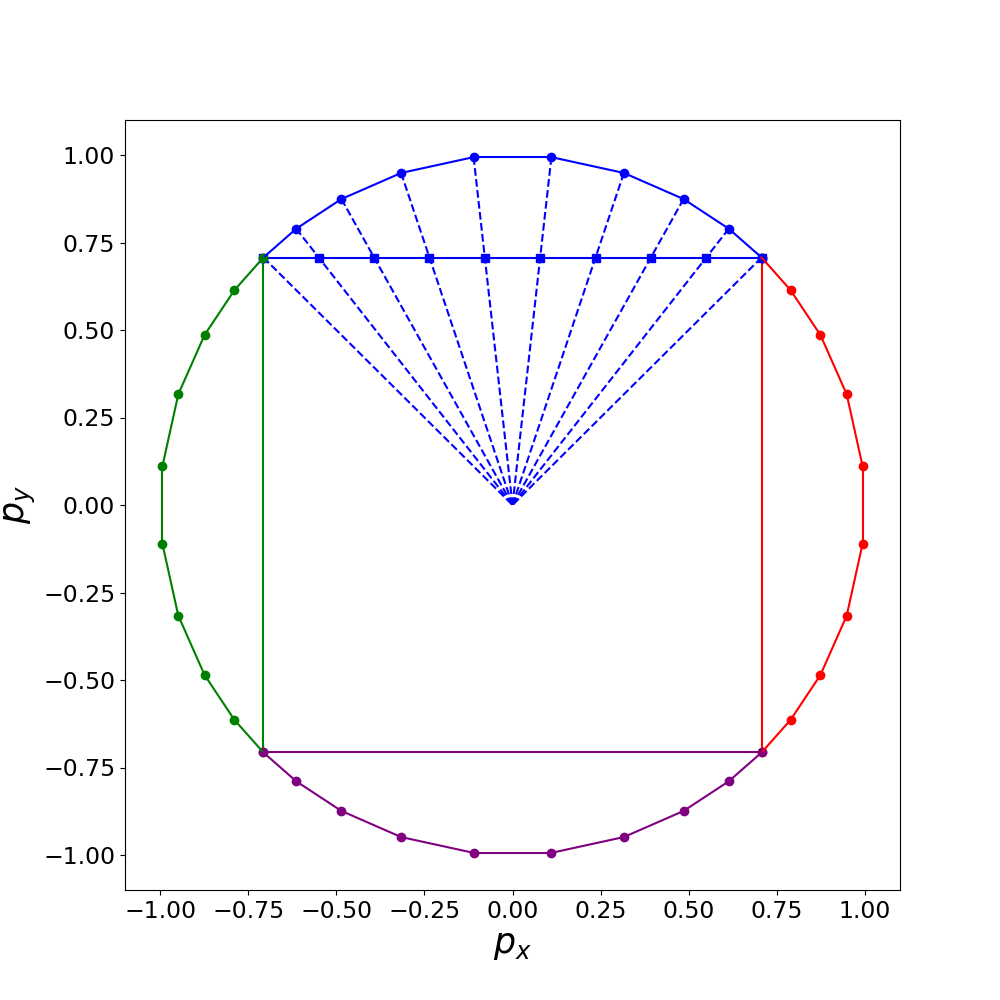
\includegraphics[width=1.1\linewidth]{g1}
		\caption{Cube and sphere equidistant mapping for $p_z=0$.\label{sph-cube-equidist}}
	\end{subfigure}


	\begin{subfigure}{0.45\textwidth}
		\centering
		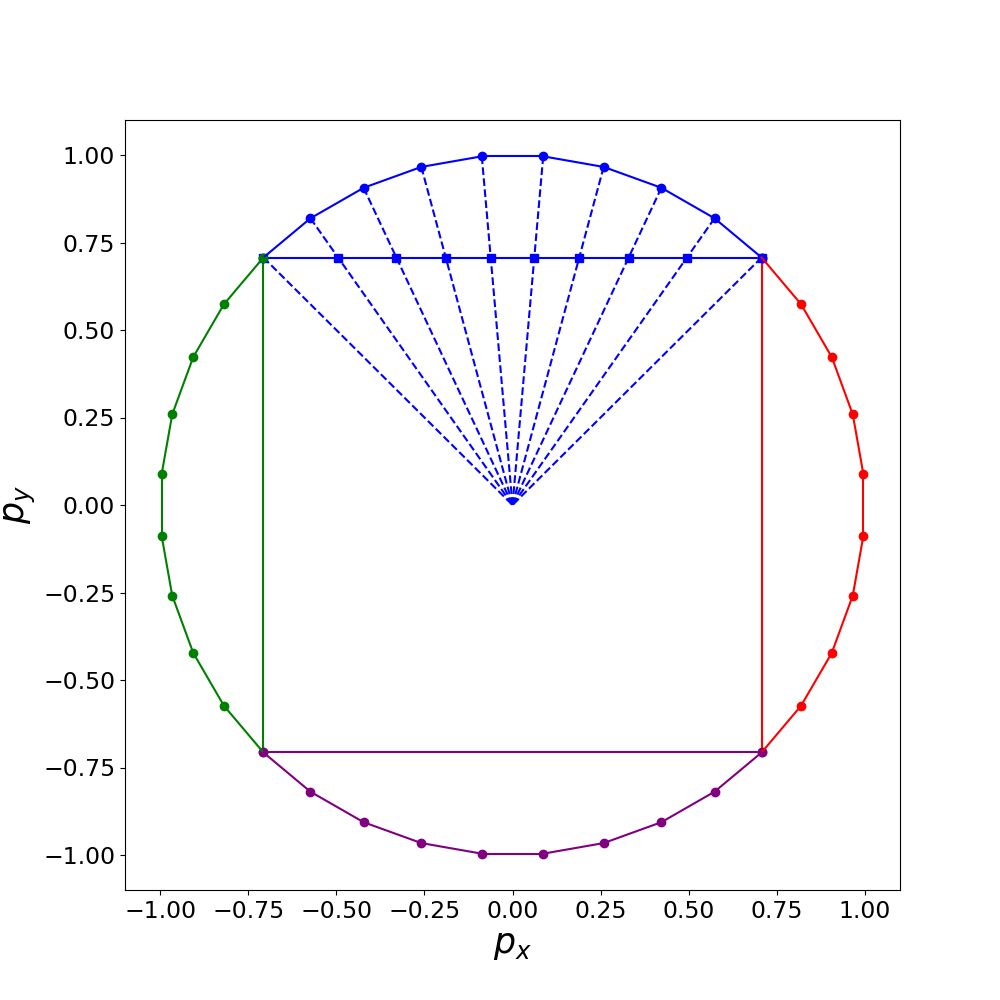
\includegraphics[width=1.1\linewidth]{g2}
		\caption{Equiangular mapping for $p_z=0$.\label{sph-cube-equiangular}}
	\end{subfigure}
	\begin{subfigure}{0.45\textwidth}
	\centering
	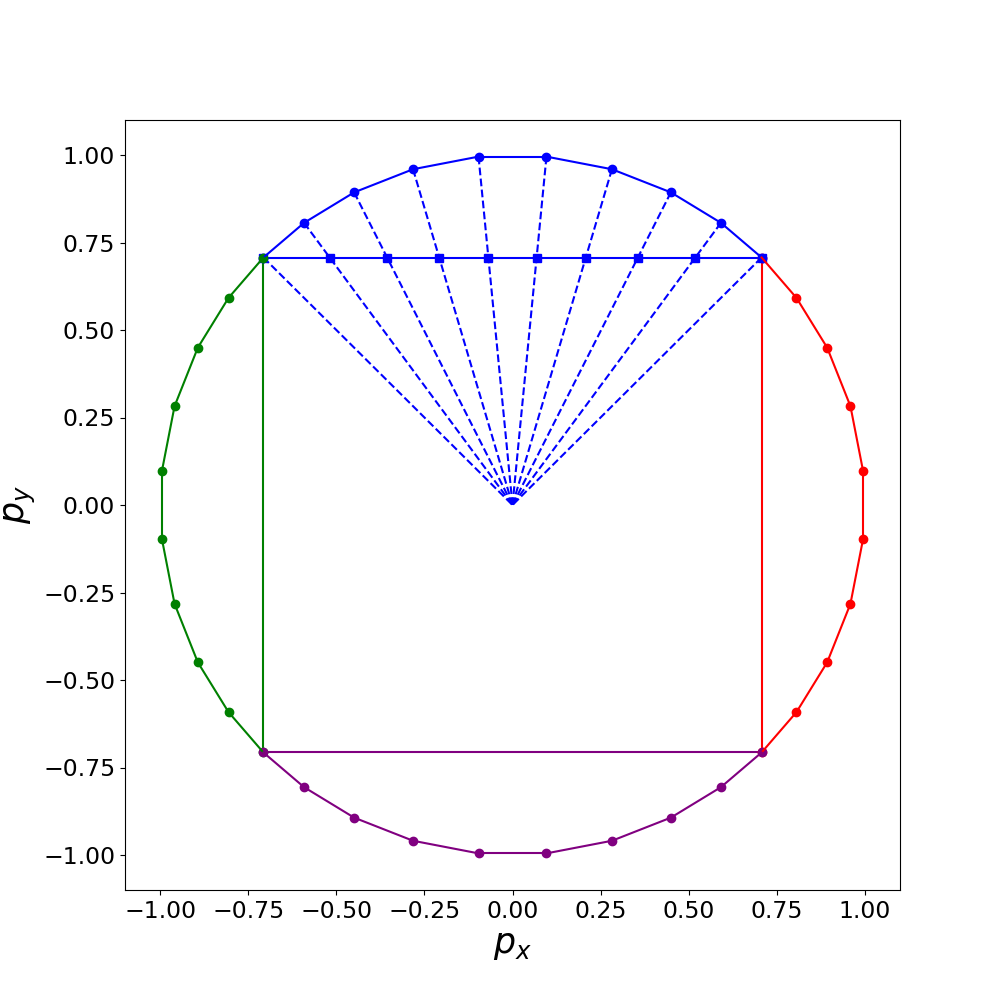
\includegraphics[width=1.1\linewidth]{g0}
	\caption{\textcolor{red}{Equi-edge mapping for $p_z=0$.}\label{sph-cube-equiedge}}
\end{subfigure}
\caption{Illustration of the cube-to-sphere projection using the equidistant (a),  equiangular (b) and the \textcolor{red}{equi-edge}  (c) mappings. This figure uses a cross section obtained with $p_z=0$.}
\label{sph-cube-mappings}
\end{figure}

The derivative of ${\Gamma}_p$ is a $3\times2$ matrix denoted by $d{\Gamma}_p$. Explicit formulas are provided in  \ref{metric_terms}.
With the aid of the derivative,  a basis of tangent vectors $\{{\partial_X {\Gamma}_p, \partial_Y {\Gamma}_p}\}$ may be defined
at each point on the sphere, where $\partial_X {\Gamma}_p$ is given by the first column of $d{\Gamma}_p$ 
and $\partial_Y {\Gamma}_p$ is given by the second column of $d{\Gamma}_p$.
Along with, the metric tensor is defined as
$G_{{\Gamma}} := (d\Gamma_p)^T \cdot d\Gamma_p$.
It is easy to see that the metric tensor does not depend on $p$.
The Jacobian of the metric tensor $G_{{\Gamma}}$ is then defined as $\sqrt{\mathfrak{g}_{{\Gamma}}} :=
\sqrt{|\det{G_{{\Gamma}}}|}.$

Let us assume that it is given a function $\beta:[-a,a] \to [-1,1]$, for some positive $a>0$,
supposed to be bijective and $\mathcal{C}^1$ with inverse $\mathcal{C}^1$ as well.
That is, $\beta$ is a change of coordinates.
Then, new cube-to-sphere mappings may be constructed.
Indeed, we may define $ {\Psi}_p: [-a,a]\times [-a,a] \to \mathbb{S}^2_R$,
given by 
\begin{equation}
	\label{psi-def}
	{\Psi}_p(x,y) := {\Gamma}_p\big(\beta(x),\beta(y)\big).
\end{equation}
Using the derivatives of ${\Psi}_p(x,y)$, a basis of tangent vectors $\{{\partial_x {\Psi}_p}, {\partial_y {\Psi}_p}\}$ induced by this mapping is defined.
The metric tensor of ${\Psi}_p$, denoted by $G_{\Psi}$, is defined as $G_{\Gamma}$, namely $G_{\Psi} = (d\Psi_p)^T d\Psi_p$.
Finally, the metric term for $\Psi$ is defined as $\sqrt{\mathfrak{g}_{\Psi}}:= \sqrt{|\det{G_{\Psi}}|}$,
which may also be expressed as
\begin{equation}
	\label{mt-sina}
	\sqrt{\mathfrak{g}_{\Psi}}(x,y) =	
	\|\partial_x  {\Psi}_p \| \|\partial_y  {\Psi}_p \| \sin \alpha(x,y,p),
\end{equation}
where $\|\cdot\|$ is the Euclidian norm of $\mathbb{R}^3$, $\alpha$ is the angle between $\partial_x {\Psi}_p$ and $\partial_y {\Psi}_p$ that
satisfies
\begin{equation}
	\label{mt-cosa}
	\cos{\alpha(x,y,p)} = {\langle
		\boldsymbol{e}_x(x,y,p),
		\boldsymbol{e}_y(x,y,p) \rangle },
\end{equation}
where $\langle \cdot, \cdot \rangle$ denotes 
the standard inner product of $\mathbb{R}^3$ and 
$\{\boldsymbol{e}_x, \boldsymbol{e}_y\}$ is the normalization of the tangent vector basis
$\{{\partial_x {\Psi}_p}, {\partial_y {\Psi}_p}\}$.

\textcolor{red}{Given a tangent vector field $\boldsymbol{u}$ on the sphere, also known as wind, we may represent it using the basis obtained by cubed-sphere coordinates:
\begin{equation}
	\label{contravariant-wind}
	\boldsymbol{u}(x, y, p) = 
	\mathfrak{u}(x, y,p ) \partial_x{\Psi}_p(x, y) + 
	\mathfrak{v}(x, y, p) \partial_y{\Psi}_p(x, y).
\end{equation}
This representation $(\mathfrak{u},\mathfrak{v})$ is known as the contravariant representation, and they are the components of the wind on the tangent basis defined by the cubed-sphere mapping.
A detailed discussion on how the cubed-sphere wind representation is related to the zonal and meridional representation is presented in \ref{ap-wind}.
In practice, FV3 schemes \cite{putman:2007, harris:2021} use the normalized contravariant wind
$({u},{v})$ given by:
\begin{equation}
	\label{norm-contravariant-wind}
	\boldsymbol{u}(x, y, p) = 
	{u}(x, y, p) \boldsymbol{e}_x(x, y, p) + 
	{v}(x, y, p) \boldsymbol{e}_y(x, y, p),
\end{equation}
where $\boldsymbol{e}_x$ and $\boldsymbol{e}_y$ are the normalized cubed-sphere tangent vectors, which may be computed easily in terms of the grid points \cite[Appendix C2]{chen:2021}.
It is easy to see that:
\begin{equation}
	\label{contra-uv}
	\mathfrak{u}(x,y,p)  = \frac{{u}(x,y,p)}{\|\partial_x{\Psi}_p(x,y)\|}, \quad
	\mathfrak{v}(x,y,p)  = \frac{{v}(x,y,p)}{\|\partial_y{\Psi}_p(x,y)\|}.
\end{equation}
Finally, we recall that the horizontal divergence operator for a  wind $\boldsymbol{u}$  on the sphere is defined in terms of the cubed-sphere metric terms as follows:
\begin{align}
	\label{div-def}
	[\nabla \cdot {\boldsymbol{u}}](x,y,p) :=
	\frac{1}{\sqrt{\mathfrak{g}_{\Psi}}(x,y)}
	\bigg(
	\partial_x(\sqrt{\mathfrak{g}_{\Psi}}\mathfrak{u})(x,y,p) +
	\partial_y(\sqrt{\mathfrak{g}_{\Psi}}\mathfrak{v})(x,y,p)
	\bigg),
\end{align}
for $x,y\in[-a,a]$, $p$ is the panel and
$\mathfrak{u}$ and $\mathfrak{v}$ are the contravariant wind components.
The divergence operator shall be used in the transport model in Section \ref{adv-2d}.
}
%%%%%%%%%%%%%%%%%%%%%%%%%%%%%%%%%%%%%%%%%%%%%%%%%%%%%%%%%%%%%%
\subsection{Equiangular mapping}
\label{cs-equiangular}
Another cubed-sphere mapping is the equiangular mapping, 
introduced by \cite{ronchi:1996}, which leads to a more uniform grid.
This mapping is obtained by considering $\beta(x) = \tan{x}$ and $a=\frac{\pi}{4}$.
In this case, $\beta(x)$ represents the angular coordinates, and the cube-sphere is obtained by partitioning the angle between
grid points equally, as illustrated in Figure \ref{sph-cube-equiangular}, hence the name equiangular.

%%%%%%%%%%%%%%%%%%%%%%%%%%%%%%%%%%%%%%%%%%%%%%%%%%%%%%%%%%%%%%
\subsection{Equi-edge mapping}
\label{cs-equiedge}
Another cubed-sphere mapping is the equi-edge proposed by
\cite{chen:2021} using $\beta(x) = \sqrt{2}\tan{x}$ and
$a=\arcsin{\big(\frac{1}{\sqrt{3}}\big)}$.
The idea behind the equi-edge mapping lies in partitioning the edges of the spherical cube equally,
and then generating the other cells, hence the name equi-edge.
Also, this mapping leads to more uniform grid cells after applying the grid stretching option of FV3 \citep{harris:2016, chen:2021}.
\textcolor{red}{This mapping is illustrated in Figure \ref{sph-cube-equiedge}}.

%%%%%%%%%%%%%%%%%%%%%%%%%%%%%%%%%%%%%%%%%%%%%%%%%%%%%%%%%%%%%%
\subsection{Cubed-sphere grid generation}
\label{cs-grid}
Let us fix two positive integers $N$ and $\nu$, where $N$ represents the number of cells in a direction and $\nu$ represents the number of ghost cell layers.
The equiangular or equi-edge mapping, denoted by $\Psi_p$, introduced previously, is considered to generate the cubed-sphere grid.
For simplicity, the metric term $\sqrt{\mathfrak{g}}_{\Psi}$ is denoted by $\sqrt{\mathfrak{g}}$.
To generate the cubed-sphere grid, the domain $[-a,a]\times[-a,a]$ is discretized using uniformly spaced points.
\begin{align}
\label{edge-coords}
x_{i+\frac{1}{2}} = -a+i\Delta x, \quad
y_{j+\frac{1}{2}} = -a+j\Delta y,
\end{align}
where $\Delta x = \Delta y = \frac{2a}{N}$, $i,j=-\nu+1,\ldots,N+1+\nu$. The center coordinates  are defined as:
\begin{align}
	\label{center-coords}
	x_{i} = \frac{x_{i+\frac{1}{2}}+x_{i-\frac{1}{2}}}{2}, \quad
	y_{j} = \frac{y_{j+\frac{1}{2}}+y_{j-\frac{1}{2}}}{2},
\end{align}
for $i,j=-\nu+1,\ldots,N+\nu$.
Notice that the mappings ${\Psi}_p$ defined before can be computed outside the range $[-a,a]$, and the cubed-sphere mapping can be applied to all these ghost cell points.
Firstly, we shall focus the attention on the interior cells; the generation of ghost cells shall be addressed in Section \ref{cs-ghost}.

\begin{figure}[!htb]
	\centering
	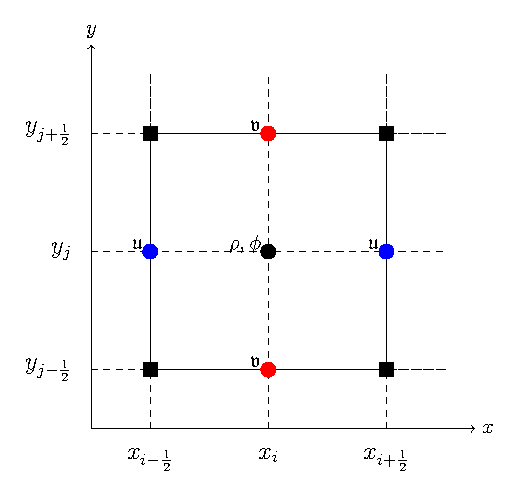
\includegraphics[width=0.5\linewidth]{fv_grid}
	\caption{
	\textcolor{red}{
	Illustration of the discrete grid indexes for a cell. 
	The corner points are depicted using black squares, while the centroids are represented using black circles. 
	The  left-right and up-down midpoints of the edges,  are illustrated in blue and red circles, respectively.
Additionally, this figure shows the positions of the contravariant wind components $\mathfrak{u}$ and $\mathfrak{v}$ in a C-grid discretization for the transport model, along with the fluid density $\rho$ and tracer concentration $\phi$ at the centers.}
	\label{cgrid}}
\end{figure}

There are four types of grid points on the cubed-sphere that are needed to be computed: the center, corners, right-left edge midpoints, and  up-down edge midpoints. 
\textcolor{red}
{These points are illustrated in Figure \ref{cgrid}.}
The corner points are computed as:
\begin{equation}
	\label{corner-points}
	\Psi_{i+\frac{1}{2},j+\frac{1}{2},p} := {\Psi}_p(x_{i+\frac{1}{2}},y_{j+\frac{1}{2}}),
\end{equation}
$i,j=0, \ldots, N$.
To ease the notation hereafter, the dependence on $p$ is omitted because it does not interfere with what is going to be discussed in this section.
Figure \ref{cs-grids-N10} shows the obtained grid lines in for $N=10$.
\begin{figure}[!htb]
	\begin{subfigure}{0.42\textwidth}
		\centering
		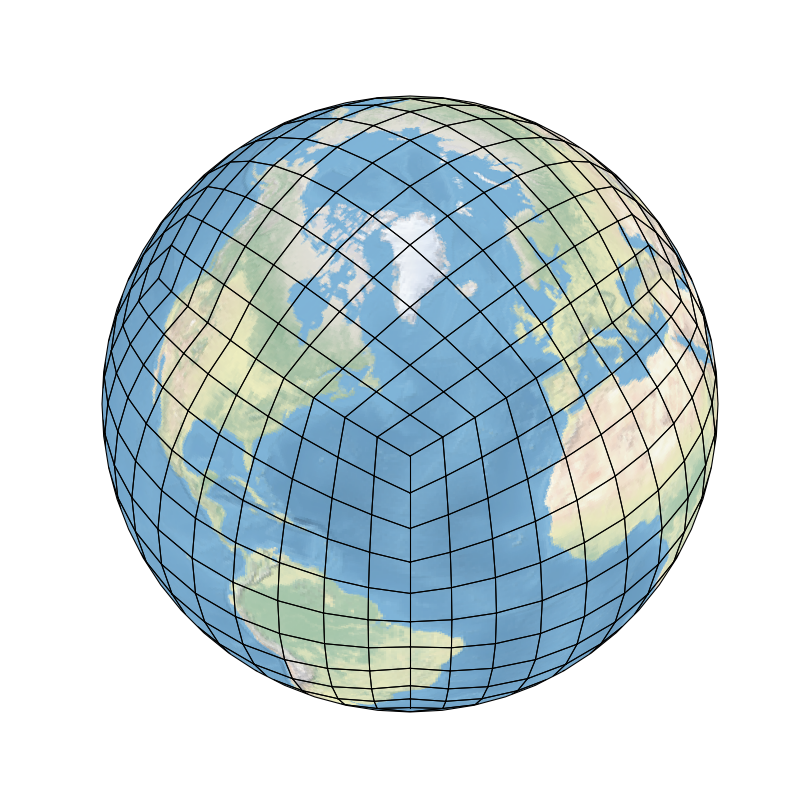
\includegraphics[width=1.1\linewidth]{gnomonic_equiedge_cs_10_sphere}
		\caption{Equiangular grid}
	\end{subfigure}
	\centering
\begin{subfigure}{0.42\textwidth}
	\centering
	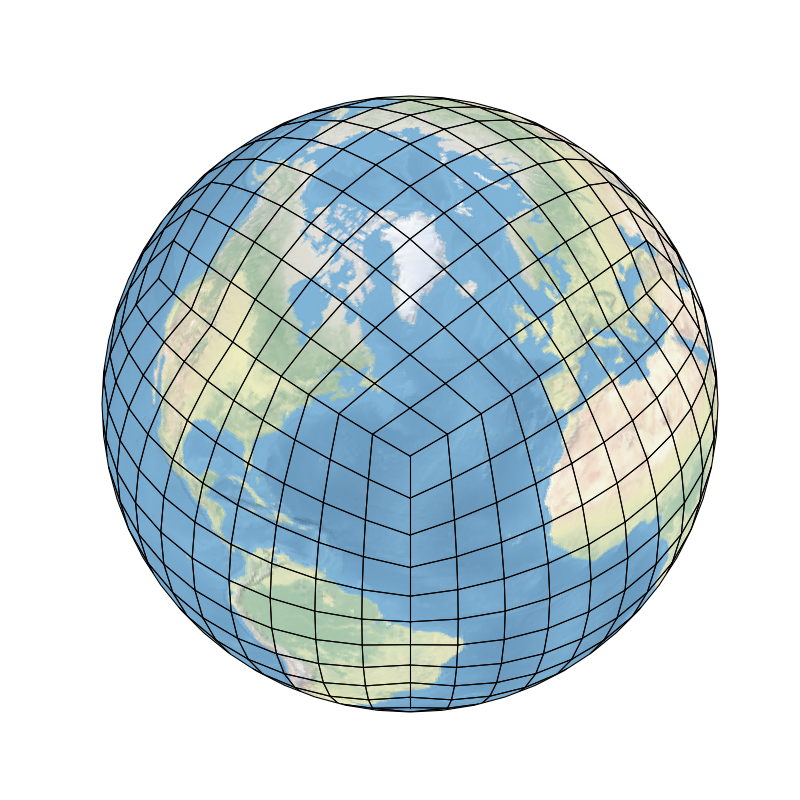
\includegraphics[width=1.1\linewidth]{gnomonic_equiangular_cs_10_sphere}
	\caption{Equi-edge grid}
\end{subfigure}
	\caption{(a) Illustration of the resulting gridlines
		for the cubed-sphere equiangular and equi-edge mapping for $N=10$.\label{cs-grids-N10}}
\end{figure}

The center, corners, right-left edge midpoints, and up-down edge midpoints could be computed similarly using Equation \eqref{corner-points}. 
However, in FV3, these points are replaced by averages of the corner points. Thus, the center points are computed by averaging the values of 4 corner points:
\begin{equation}
	\Psi_{ij} :=
	R
	\frac{\Psi_{i+\frac{1}{2},j+\frac{1}{2}} + \Psi_{i+\frac{1}{2},j-\frac{1}{2}} + \Psi_{i-\frac{1}{2},j+\frac{1}{2}} + \Psi_{i-\frac{1}{2},j-\frac{1}{2}}}
	{\|\Psi_{i+\frac{1}{2},j+\frac{1}{2}} + \Psi_{i+\frac{1}{2},j-\frac{1}{2}} + \Psi_{i-\frac{1}{2},j+\frac{1}{2}} + \Psi_{i-\frac{1}{2},j-\frac{1}{2}}\|}.
\end{equation}
Similarly, the right-left edge points $\Psi_{i+\frac{1}{2},j}$ are obtained by averaging the values of 2 corner points
and the up-down edge points  $\Psi_{i,j+\frac{1}{2}}$ are also  given by the average of 2 corner points.
It is easy to see that generating the grid points using these averages has an $\mathcal{O}(\Delta x^2)$ difference compared to generating these points using a cubed-sphere mapping ${\Psi}_p$.

%%%%%%%%%%%%%%%%%%%%%%%%%%%%%%%%%%%%%%%%%%%%%%%%%%%%%%%%%%%%%%
The following geodesic distances in $x$ and $y$ directions, respectively, are introduced:
\begin{align}
	\label{distcube}
	{\delta} x_{ij} = d(\Psi_{i+\frac{1}{2},j},\Psi_{i-\frac{1}{2},j}) , \quad
	{\delta} y_{ij} = d(\Psi_{i,j+\frac{1}{2}},\Psi_{i,j-\frac{1}{2}}),
\end{align}
where $d(P,Q) = R\arccos{(\langle P, Q \rangle)}$, for $P,Q \in \mathbb{S}^2_R$.
These distances may be represented in terms of the tangent vector norms as:
\begin{align}
	{\delta} x_{ij} = 
	\int_{x_{i-\frac{1}{2}}}^{x_{i+\frac{1}{2}}}
	\|\partial_x  {\Psi}_{p}\|(x,y_j) \,dx ,\quad
	{\delta} y_{ij} =
	\int_{y_{j-\frac{1}{2}}}^{y_{j+\frac{1}{2}}}
	\|\partial_y {\Psi}_{p}\|(x_i,y) \,dy.
\end{align}
Hence, their midpoint approximations are defined as:
\begin{align}
	\label{distcube2}
	\hat{\delta} x_{ij} = \|\partial_x {\Psi}_{p}(x_i,y_j)  \|\Delta x,\quad
	\hat{\delta} y_{ij} = \|\partial_y {\Psi}_{p}(x_i,y_j) \|\Delta y.
\end{align}
We point out that $\hat{\delta} x_{ij}$ and $\hat{\delta} y_{ij}$ are replaced in FV3 code by the geodesic distances that they approximate whenever they appear, which are second-order accurate by the midpoint rule.
A control volume of the cubed-sphere is denoted by $\Omega_{ijp}$, defined as $\Omega_{ijp} = {\Psi}_p(\Omega_{ij})$.
The area of $\Omega_{ijp}$ is denoted by $|\Omega_{ij}|$,
since the area does not depend on the panel due to the grid symmetry.
The control volume area may be expressed as:
\begin{equation}
	\label{area}
	|\Omega_{ij}| = \int_{x_{i-\frac{1}{2}}}^{x_{i+\frac{1}{2}}} \int_{y_{j-\frac{1}{2}}}^{y_{j+\frac{1}{2}}}{\sqrt{\mathfrak{g}}(x,y)} \,dx \,dy = 
	|\hat{\Omega}_{ij}| + \mathcal{O}(\Delta x^2),
\end{equation}
where 
\begin{equation}
	\label{area2}
	|\hat{\Omega}_{ij}| = \sqrt{\mathfrak{g}}_{ij} \Delta x \Delta y,
\end{equation} $\sqrt{\mathfrak{g}}_{ij}=\sqrt{\mathfrak{g}}(x_i,y_j) $
and the last equality in Equation \eqref{area} follows from the midpoint rule for integration.
Similar to the grid lengths, the approximated areas $|\hat{\Omega}_{ij}|$ are replaced by the exact area $|\Omega_{ij}|$ in the FV3 code.
\begin{table}[htbp]
	\centering
	\caption{Mean length, minimum length, and maximum length for different values of $N$ considering the equiangular grid.\label{g2-dx-table}}
	\begin{tabular}{|c|c|c|c|c|c}\hline
		$N$ & Mean Length (km) & Min Length (km) & Max Length (km) & $\frac{\text{Max}}{\text{Min}}$ \\ \hline
		48 & 220 & 202 & 240 & 1.1890 \\
		96 & 109 & 99 & 118  & 1.1892 \\
		192 & 54 & 49 & 59  & 1.1892 \\
		384 & 27 & 24 & 29  & 1.1892 \\
		768 & 13 & 12 & 14  & 1.1892\\
		\hline
	\end{tabular} 
\end{table}
\begin{table}[htbp]
	\centering
	\caption{As Table \ref{g2-dx-table} but considering the equi-edge grid. \label{g0-dx-table}}
	\begin{tabular}{|c|c|c|c|c|c}\hline
		$N$ & Mean Length (km) & Min Length (km) & Max Length (km) & $\frac{\text{Max}}{\text{Min}}$ \\ \hline 
		48 & 218 & 175 & 266 & 1.5192 \\
		96 & 108 & 86 & 131 & 1.5195 \\
		192 & 54 & 43 & 65 & 1.5196 \\
		384 & 26 & 21 & 32 & 1.5197 \\
		768 & 13 & 10 & 16 & 1.5197 \\
		\hline
	\end{tabular}
\end{table}

Tables  \ref{g2-dx-table} and \ref{g0-dx-table} display the lengths of the  equiangular and equi-edge grids for $N=48\times 2^k$, 
where $k = 0,\ldots, 4$. These values of $N$ are considered in this work.
It can be observed that in terms of length of the cells, the equi-edge grid is less uniform than the equiangular grid.
Despite this, the equi-edge grid is the operational grid in some applications of FV3 \cite{harris:2021,chen:2021}, such as, for instance, 
the Next Generation Global Prediction System (NGGPS) \cite{zhou:2019}, 
because this grid is expected to produce less grid imprinting due to its greater uniformity near the cubed edges.

\subsection{Ghost cells}
\label{cs-ghost}
Currently, FV3 uses the cells of the adjacent panels as ghost cells, employing an approach named kinked grid by \cite{mouallem:2023}. 
This was the approach used by \cite{putman:2007}.
In this work, we shall use the extended grid lines of the cubed-sphere mapping to generate the ghost cells, in an approach named duo-grid recently introduced by \citep{chen:2021}. This approach was recently exploited in FV3 by \cite{mouallem:2023} and helps to reduce grid imprinting.
\begin{figure}[!htb]
	\centering
	\begin{subfigure}{0.49\textwidth}
		\centering
		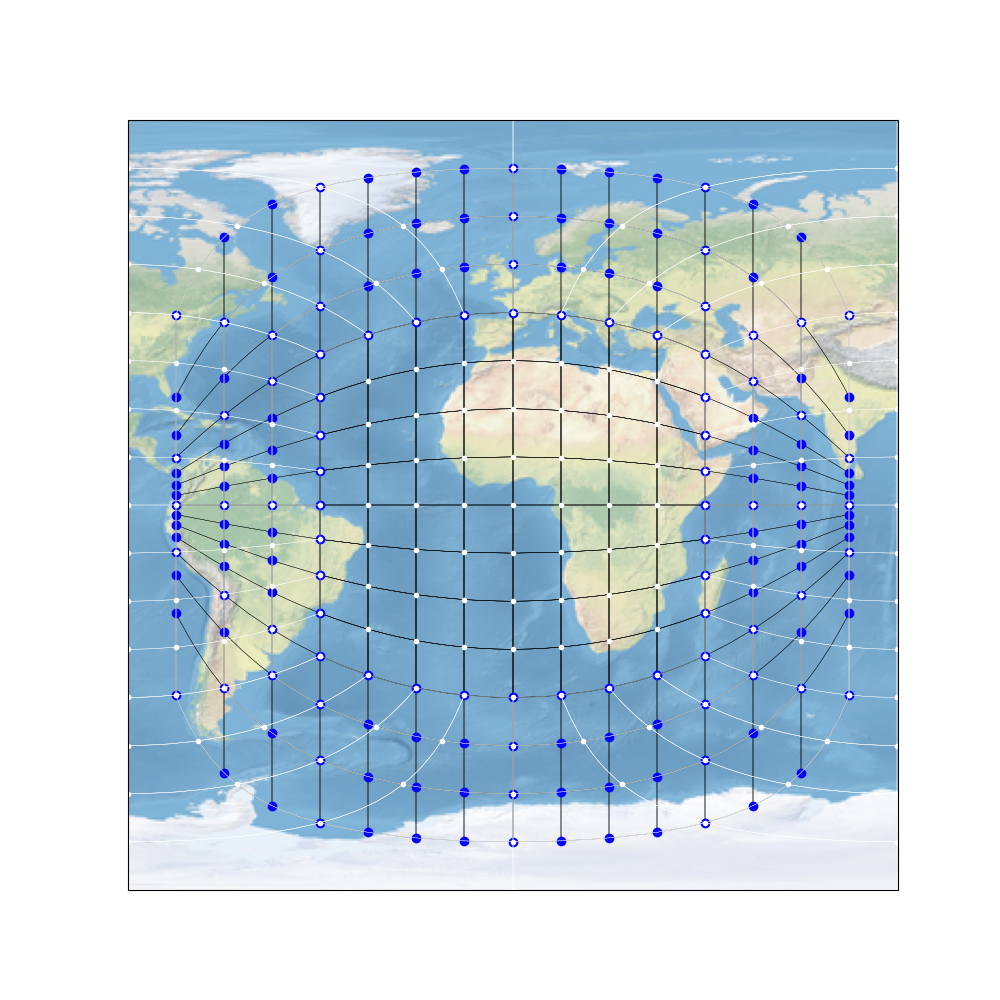
\includegraphics[width=1.13\linewidth]{g2_duo}
		\caption{Extended equiangular grid.\label{cs-duo-g2}}
	\end{subfigure}
	\begin{subfigure}{0.49\textwidth}
		\centering
		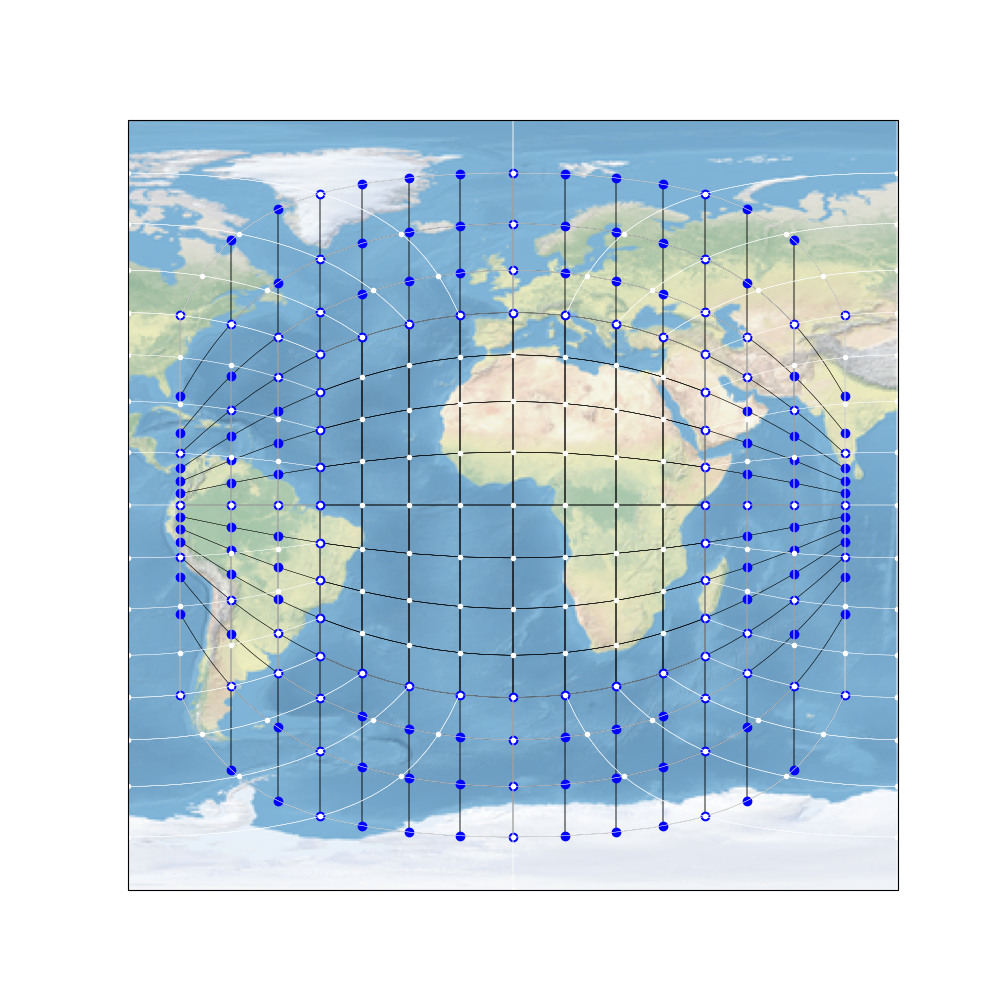
\includegraphics[width=1.13\linewidth]{g0_duo2}
		\caption{Mirrored equi-edge grid.\label{cs-duo-g02}}
	\end{subfigure}
	\caption{Grid lines of panel 1, including ghost cells, for the extended equiangular grid (a) and the mirrored equi-edge grid (b).
		Corner ghost points are denoted by blue circles, and the corner interior points are denoted by white points.\label{cs-duo}}
\end{figure}

The corner ghost cell points are generated by applying Equation \eqref{corner-points} for $i$ and $j$ out of the range $0$ to $N+1$. 
The other grid points are again computed by averaging the corner points, as in the interior grid points.
Figure \ref{cs-duo-g2} show how the corner ghost points of the equiangular grid are aligned on common geodesics of the adjacent panels.
This property has been known since the work of \cite{ronchi:1996}.

%\begin{figure}[!htb]
%	\centering
%	\begin{subfigure}{0.4\textwidth}
%		\centering
%		\includegraphics[width=0.7\linewidth]{duoscalar1}
%		\caption{Center values (blue circles).\label{cs-duoscalar-1}}
%	\end{subfigure}
%	\begin{subfigure}{0.4\textwidth}
%		\centering
%		\includegraphics[width=0.7\linewidth]{duoscalar2}
%		\caption{Adjacent values (red and green circles)\label{cs-duoscalar-2}}
%	\end{subfigure}
%	
%	\begin{subfigure}{0.4\textwidth}
%		\centering
%		\includegraphics[width=0.7\linewidth]{duoscalar3}
%		\caption{Ghost cell values (blue squares)\label{cs-duoscalar-3}}
%	\end{subfigure}
%	\begin{subfigure}{0.4\textwidth}
%		\centering
%		\includegraphics[width=0.7\linewidth]{duoscalar4}
%		\caption{Interpolation lines (dashed blue lines)\label{cs-duoscalar-4}}
%	\end{subfigure}
%	\caption{Illustration of the ghost cell interpolation for a scalar field given at cell centers. \label{cs-duoscalar}}
%\end{figure}

The extended grid alignment property is very useful because it allows us to use 1D Lagrange interpolation to estimate the function values at the ghost cells using function values from neighboring panels, and it has been widely used in the literature \cite{ross:2006, croisille:2013,katta:2015,katta:2015b, chen:2021}. 
A complete description of this process has been provided by \cite{zerroukat:2022}. %, and we illustrate the idea in Figure \ref{cs-duoscalar}, assuming that we have the values of a function at the cell centers.
However, the analogous property does not hold for the equi-edge grid.
To address this problem, \cite{chen:2021} proposes modifying the ghost values of the $x$ and $y$ coordinates by mirroring certain points. 
This generates the new ghost points, aligning them on the same geodesic as those from the neighboring panel, as illustrated in Figure \ref{cs-duo-g02}.
More formally, for $g=1,2,\ldots,\nu$, the mirrored values are given by:
\begin{align}
	\hat{x}_{-g+\frac{1}{2}}  &= \arctan\left(\frac{1}{a}\tan\left(-\frac{\pi}{2}-\arctan{(a \tan{x_{g+\frac{1}{2}} })}\right)\right),
\end{align}
and	$\hat{x}_{N+g+\frac{1}{2}} = -\hat{x}_{-g+\frac{1}{2}}$
to replace ${x}_{-g+\frac{1}{2}},{x}_{N+g+\frac{1}{2}}$, respectively.
Similar formulas are used for the $y$ component.


%% The Appendices part is started with the command \appendix;
%% appendix sections are then done as normal sections

\section{The conservative transport equation on the cubed-sphere}
\label{adv-2d}
The goal of this section is to present and solve numerically the conservative transport equation on the cubed-sphere. 
We are going to consider the equi-edge or equiangular cubed-sphere mappings $\Psi_p$ and their respective local coordinates $(x,y)$.
\textcolor{red}{Once again, the metric term is denoted by $\sqrt{\mathfrak{g}}_{\Psi}$ by $\sqrt{\mathfrak{g}}$ for simplicity.}
Following \cite{nair:2010}, the transport model without sources or sinks is considered:
\begin{align}
	\label{transp-rho}
	[\partial_t \rho + \nabla \cdot (\rho \boldsymbol{u})](x,y,p,t)&=0,\\
	\label{transp-phi}
	[\partial_t (\rho \phi) + \nabla \cdot (\rho \phi \boldsymbol{u})](x,y,p,t)&=0,
\end{align}
for $x,y\in[-a,a]$, $t \in [0,T]$, where $T$ is the final time,
\textcolor{red}
{$\boldsymbol{u}$ is the wind, $\mathfrak{u}$ and $\mathfrak{v}$ are the contravariant wind components (Equation \ref{contravariant-wind}),
$\rho$ is the fluid density and $\phi$ is the tracer concentration}.
Additionally, for the transport model, it is assumed that the initial conditions are given as $\rho(x,y,p,0)=\rho_0(x,y,p)$ and $\phi(x,y,p,0)=\phi_0(x,y,p)$, given $\rho_0$ and $\phi_0$. % and that the boundary conditions are related to the cubed-sphere topology.
Equation \eqref{transp-rho} is the continuity equation and Equation \eqref{transp-phi} is the conservative advection equation.
In this framework, $\rho \phi$ represents the tracer density, and the total masses of $\rho$ and $\rho \phi$ are preserved.  Therefore, these quantities are referred to as conserved quantities.

In the transport model, one can easily see that the tracer variable $\phi$ is advected.
That is, $\phi$ satisfies the non-conservative advection equation:
\begin{align}
	\label{adv-phi}
	[\partial_t \phi +  
	\langle\boldsymbol{u}, \nabla \phi \rangle](x,y,p,t)&=0.
\end{align}
Equations \eqref{transp-rho} and \eqref{transp-phi} have the same form. 
\textcolor{red}{Hence, it follows from the definition of the divergence operator in terms of the cubed-sphere mapping (Equation \eqref{div-def}) that the equation that needs to be solved may be uniquely expressed as:}
\begin{equation}
	\label{2d-adv}
	[{\partial_t (\sqrt{\mathfrak{g}}q)}+
	{\partial_x (\mathfrak{u}\sqrt{\mathfrak{g}}q)}+
	{\partial_y (\mathfrak{v}\sqrt{\mathfrak{g}}q)}]
	(x, y, p, t) = 0,
\end{equation}
where $q=\rho$ or $q=\rho \phi$. 
Additionally, it is assumed that $q(x,y,p,0)=q_0(x,y,p)$ for some given $q_0$.
Equation \eqref{2d-adv} is referred to as the conservative transport equation.
The goal now is to solve Equation \eqref{2d-adv}, which will allow for the solution of the transport model on the sphere.
In the shallow-water model, Equation \eqref{2d-adv} is satisfied for the fluid depth and the absolute vorticity.

For simplicity, the dependence on the panel $p$ is omitted as the discussion here does not depend on $p$.
Initially, the time is discretized by introducing the time step $\Delta t = \frac{T}{N_T}$, for some integer $N_T > 0$, and  the discrete time instants are given by $t^n = n\Delta t$,
for $n=0,\ldots,N_T$. 
We are particularly interested in proposing a scheme that approximates the values of $q(x_i,y_j,t^n)$ for $i,j=1,\ldots,N$ and $n=1,\ldots,N_T$, where the numerical approximation is denoted  by $q_{ij}^n$.
It is assumed, of course, that $q_{ij}^0 = q(x_i,y_j,0)$.

Assuming that the values $q_{ij}^n$ for $i,j=1, \ldots, N$ are given, we are going to use the dimension-splitting approach as discussed in \cite{lin:1996} to obtain $q_{ij}^{n+1}$. 
Beforehand, the ghost cell interpolation method described in Section \ref{cs-ghost} is used on the grid function $q^n$, so  the values $q_{ij}^n$ for $i,j=-\nu+1, \ldots, N+\nu$ are obtained.

The scheme proposed by \cite{lin:1996} is based on replacing the two-dimensional conservative transport equation (Equation \eqref{2d-adv}) by combining the solutions of the conservative transport equation when considering only the $x$ direction and then separately when considering only the $y$ direction.
More precisely, $N+2\nu$ one-dimensional conservative transport equations in the $x$-direction are considered:
\begin{equation}
	\label{1d-adv-xdir}
	[{\partial_t (\sqrt{\mathfrak{g}}q^x)}+{\partial_x (\mathfrak{u}\sqrt{\mathfrak{g}}q^x)}](x, y_j, t) = 0,
\end{equation}
for $j=-\nu+1, \ldots, N + \nu$, and
$N+2\nu$ one-dimensional conservative transport equations in the $y$-direction
\begin{equation}
	\label{1d-adv-ydir}
	[{\partial_t (\sqrt{\mathfrak{g}}q^y)} +{\partial_y (\mathfrak{v}\sqrt{\mathfrak{g}}q^y)}](x_i, y, t) = 0,
\end{equation}
for $i=-\nu+1, \ldots, N + \nu$, using $q_{ij}^n$ as initial data.
Therefore, the solution to the 1D conservative transport equation needs to be specified.
A finite-volume approach is going to be used to solve Equations \eqref{1d-adv-xdir} and \eqref{1d-adv-ydir}, as described in the next subsection.

\textcolor{red}
{
The goal now is to describe the details of the numerical method proposed by \citep{putman:2007}, known as the FV3 scheme, currently used in FV3.
In each part of the FV3 method that will described, we will propose modifications aimed at improvements. 
Additionally, the scheme proposed in this work is named LT2.
The justification for its name will be provided in the next sections, as it utilizes an average of two Lie-Trotter splittings \cite{holden:2010}, along with a second-order Runge-Kutta method for the departure point equation.
}

\subsection{The one-dimensional finite-volume discretization}
\label{1d-adv}
This subsection is dedicated to describing the 1D finite-volume scheme for solving the conservative transport equation separately in the $x$ and $y$ directions.
The description here will only consider the conservative transport equation in the $x$ direction (Equation \ref{1d-adv-xdir}), but everything here generalizes straightforwardly to the conservative transport equation in the $y$ direction.

For each $j=-\nu+1, \cdots, N+\nu$ fixed, the following linear conservative transport equation in the conservative form is considered:
\begin{equation}
	\label{1d-avd-eq}
	\begin{cases}
		[{\partial_t (\sqrt{\mathfrak{g}} {q})} + {\partial_x (\mathfrak{u}\sqrt{\mathfrak{g}}{q}})](x, t)
		= 0, \quad \forall (x,t) \in [-a, a]\times [0,T],\\
		q(x,0) = q_0(x), \quad \forall x \in [-a, a].
	\end{cases}
\end{equation}
where the notation abuses $\sqrt{\mathfrak{g}}(x) = \sqrt{\mathfrak{g}}(x,y_j)$ and $\mathfrak{u}(x,t) = \mathfrak{u}(x,y_j,t)$ are being used, along with the notations $\sqrt{\mathfrak{g}}_i = \sqrt{\mathfrak{g}}(x_i,y_j)$ and ${\mathfrak{u}}_{i+\frac{1}{2}}^n = {\mathfrak{u}}(x_{i+\frac{1}{2}},y_j,t^n)$.
Furthermore, the dependence on $j$ is omitted to ease notation.
The average values in the $x$ direction for the $i$-th cell are defined as:
\begin{equation}
	\label{1d-average-def}
	\overline{(\sqrt{\mathfrak{g}}q)}_{i}(t) = \frac{1}{\Delta x} \int_{x_{i-\frac{1}{2}}}^{x_{i+\frac{1}{2}}} {(\sqrt{\mathfrak{g}}q)}(x,t) \,dx.
\end{equation}
Following the finite-volume approach as in \cite{leveque:1990},
Equation \eqref{1d-avd-eq} is integrated in space on 
$[x_{i-\frac{1}{2}},x_{i+\frac{1}{2}}]$
followed by an integration in time on $[t^{n},t^{n+1}]$, leading to the integral version of the \textcolor{red}{conservative transport equation}:
\begin{equation}
	\label{1d-adv-integral}
	\overline{(\sqrt{\mathfrak{g}}q)}_i(t^{n+1}) =  \overline{(\sqrt{\mathfrak{g}}q)}_i(t^{n}) -
	\frac{\Delta t}{\Delta x}
	\frac{\delta_x}{\Delta t}\bigg(
	\int_{t^{n}}^{t^{n+1}}
	{(\mathfrak{u}{\sqrt{\mathfrak{g}}q})}(x_i, t) \,dt \bigg),
\end{equation}
$ \forall i = 1, \ldots, N,$ $\forall n = 0, \ldots, N_T-1$
and $\delta_x \varphi(x_i) = \varphi(x_{i+\frac{1}{2}})-\varphi(x_{i-\frac{1}{2}})$, for any function $\varphi$.
It is important to note that no approximations have been made in Equation \eqref{1d-adv-integral}. 
Equation \eqref{1d-adv-integral} needs to approximate the time-averaged flux at the cell edges $x_{i\pm\frac{1}{2}}$
to derive a finite-volume scheme. This flux, in principle, requires knowledge of $q$ over the entire interval $[t^n, t^{n+1}]$. 
To overcome this, the temporal integral is expressed as a spatial integral at time $t^n$. 
This approach avoids the need for information about $q$ throughout the entire interval $[t^n, t^{n+1}]$. 
Furthermore, this spatial integral domain is closely related to the definition of the departure point. 

To introduce the definition of departure point, for each $s \in [t^n,t^{n+1}]$,
the following Cauchy problem backward in time is introduced:
\begin{equation}
	\label{1d-dp-equation}
	\begin{cases}
		{\partial_t} x_{i+\frac{1}{2}}^d(t,s) = \mathfrak{u}\big(  x_{i+\frac{1}{2}}^d(t,s),t\big),\quad t\in[t^{n},s] \\
		x_{i+\frac{1}{2}}^d(s,s) = x_{i+\frac{1}{2}}.
	\end{cases}
\end{equation}
The point $ x_{i+\frac{1}{2}}^d(t^n,s)$ is called departure point at time $t^n$
of the point $x_{i+\frac{1}{2}}$ at time $s$.
In Theorem \ref{flux-theorem} from \ref{app-flux}, it is shown that:
\begin{equation}
	\label{1d-avflux-eq1}
	\int_{t^n}^{t^{n+1}} (\mathfrak{u}\sqrt{\mathfrak{g}}q)(x_{i+\frac{1}{2}}, s) \,ds = 
	\int^{x_{i+\frac{1}{2}}}_{ x_{i+\frac{1}{2}}^d(t^n,t^{n+1})} (\sqrt{\mathfrak{g}}q)(x,t^n)\,dx.
\end{equation}
Therefore, replacing Equation \eqref{1d-avflux-eq1} in Equation \eqref{1d-adv-integral},
it is clear that at each time step, the values of $\overline{(\mathfrak{\sqrt{g}}q)}_{i}(t^{n+1})$ are computed based on $\overline{(\mathfrak{\sqrt{g}}q)}_{i}(t^{n})$  and the integrals 
of ${(\mathfrak{\sqrt{g}}q)}(x,t^n)$ over specific intervals that are defined by the departure points.
To perform these computations, the departure points from the edges of all control volumes are needed to calculate the required integrals.
This idea serves as the motivation for defining finite-volume Semi-Lagrangian schemes, also known as flux-form Semi-Lagrangian schemes, as explored by \cite{lin:1996}.
These schemes involve estimating the departure points and reconstructing the function ${\mathfrak{\sqrt{g}}q}$ at time $t^n$ using their average values $\overline{(\mathfrak{\sqrt{g}}q)}_{i}(t^n)$, which enables the computation of the necessary integrals.
Therefore, this serves as motivation to look for a scheme of the form:
\begin{equation}
	\label{fv-scheme}
	\overline{(\sqrt{\mathfrak{g}}q)}^{n+1}_{i} = \overline{(\sqrt{\mathfrak{g}}q)}^{n}_{i} - \frac{\Delta t}{\Delta x}
	\bigg({F}_{i+\frac{1}{2}}-{F}_{i-\frac{1}{2}}\bigg),
\end{equation}
for $i=1,\ldots,N$,
where 
\begin{equation}
	\label{numerical-flux}
	{F}_{i+\frac{1}{2}} =
	 \frac{1}{\Delta t}\int_{\tilde{x}_{i+\frac{1}{2}}^n}
	 ^{x_{i+\frac{1}{2}}}
	 (\widetilde{\sqrt{\mathfrak{g}}{q}})(x, t^n) \,dx,
\end{equation} 
is the numerical flux, where $\widetilde{(\sqrt{\mathfrak{g}}{q})}$ is a subgrid reconstruction function of $\sqrt{\mathfrak{g}}{q}$ using the average values $\overline{(\sqrt{\mathfrak{g}}q)}^{n}_{i}$ and $\tilde{x}_{i+\frac{1}{2}}^n$, which is the estimated departure point obtained by solving numerically Equation \eqref{1d-dp-equation}.
Since the Courant-Friedrichs-Lewy (CFL) condition is assumed in this work, this integral shall be constrained to a single cell, namely $[x_{i-\frac{1}{2}},x_{i+\frac{1}{2}}]$ or $[x_{i+\frac{1}{2}},x_{i+\frac{3}{2}}]$\textcolor{red}{, as will be discussed in detail in Section \ref{timeav-cfl}.
This scheme allows for the use of large time steps, as discussed in \cite{lin:1996,chen:2017}, but it is not considered in this work, since the FV3 discretization assumes the CFL condition.}

In practice, the scheme from Equation \eqref{fv-scheme} is replaced by using the midpoint rule for integration, that is $\overline{(\sqrt{\mathfrak{g}}q)}_{i}^n \approx q_{i}^n\sqrt{\mathfrak{g}}_{i}$, and therefore the scheme becomes a method to update cell center values, namely:
\begin{equation}
	\label{fv-scheme-mdp}
	{q}^{n+1}_{i} = {q}^{n}_{i} - \frac{\Delta t \Delta y}{|\hat{\Omega}_{ij}|}
	\bigg({F}_{i+\frac{1}{2}}-
	{F}_{i-\frac{1}{2}}\bigg),
\end{equation}
where we used Equation \eqref{area2}.

\subsection{One-dimensional departure point computation}
Integrating Equation $\eqref{1d-dp-equation}$ over the interval $[t,s]$, yields:
\begin{equation}
	\label{dp-integral}
	x_{i+\frac{1}{2}}^d(t,s) = x_{i+\frac{1}{2}} - \int_{t}^{s}{\mathfrak{u}}\big( x_{i+\frac{1}{2}}^d(\theta,s), \theta\big) \,d\theta.
\end{equation}
Therefore, the estimated departure point, denoted by $\tilde{x}_{i+\frac{1}{2}}^n$, takes the form:
\begin{equation}
	\label{dp-estimated}
	\tilde{x}_{i+\frac{1}{2}}^n = x_{i+\frac{1}{2}} - {\tilde{\mathfrak{u}}}^{M}_{i+\frac{1}{2}}\Delta t,
\end{equation}
where $M$ stands for the employed method.
When the FV3 method is used, $M=\text{FV3}$; when the new scheme is used, $M=\text{LT2}$. This notation shall be used for the remainder of this work.

One possible way to estimate the departure point, which is used in FV3, is:
\begin{equation}
	\label{dp-fv3}
	\tilde{\mathfrak{u}}^{FV3}_{i+\frac{1}{2}} = \mathfrak{u}^{n+\frac{1}{2}}_{i+\frac{1}{2}},
\end{equation}
which leads to a first-order accurate scheme in time.

To achieve second-order accuracy in time, a second-order Runge-Kutta (RK2) method may be employed to integrate Equation \eqref{1d-dp-equation}. Following \cite{durran:2010}, this scheme results in:
\begin{equation}
	\label{rk2-wind}
	\tilde{\mathfrak{u}}^{LT2}_{i+\frac{1}{2}} =
	\begin{cases}
		\big(1-\alpha_{i+\frac{1}{2}}^n \big)\mathfrak{\mathfrak{u}}^{n+\frac{1}{2}}_{i+\frac{1}{2}} +
		\alpha_{i+\frac{1}{2}}^n \mathfrak{u}^{n+\frac{1}{2}}_{i-\frac{1}{2}} & \text{if } {\mathfrak{u}}^n_{i+\frac{1}{2}}\geq 0,\\
		-\alpha_{i+\frac{1}{2}}^n \mathfrak{u}^{n+\frac{1}{2}}_{i+\frac{3}{2}} + \big(1+\alpha_{i+\frac{1}{2}}^n\big)
		\mathfrak{u}^{n+\frac{1}{2}}_{i+\frac{1}{2}} & \text{if } {\mathfrak{u}}^n_{i+\frac{1}{2}} < 0,\
	\end{cases}
\end{equation}
where $$\alpha_{i+\frac{1}{2}}^n =  \frac{\mathfrak{u}_{i+\frac{1}{2}}^n\Delta t}{2\Delta x}.$$
\textcolor{red}{
Notice that, in order for the linear interpolation of Equation \eqref{rk2-wind} to make sense, it is necessary to ensure that $|\alpha_{i+\frac{1}{2}}^n| \in [0,1]$. 
This requirement is particularly fulfilled when the CFL number is less than one, as discussed in Section \ref{timeav-cfl}.}
The LT2 scheme requires the wind at two time levels, while FV3 uses only one time level. 
Since this work performs simulations with prescribed winds, it is  assumed that the wind is known at time levels $n$ and $n+\frac{1}{2}$.
However, in the FV3 shallow-water solver, the C-grid step first takes the D-grid wind and convert it to a C-grid wind at time level $n$, and then the  C-grid wind at the time level $n+\frac{1}{2}$ is computed.
Therefore, considering the horizontal solver, the LT2 scheme will use information that is already available by the shallow-water solver.

\subsection{The time-averaged and upwind CFL number}
\label{timeav-cfl}
In order to compute the integral in Equation \eqref{numerical-flux}, it will be useful to introduce the time-averaged CFL number at the edges.
This integral in FV3 is expressed in terms of this number.
For the LT2 scheme, the CFL number at the edges is defined naturally as
\begin{align}
	\label{cfl_LT2}
	\tilde{c}_{i+\frac{1}{2}}^{LT2} = {\mathfrak{\tilde{u}}}_{i+\frac{1}{2}}^{LT2}\frac{\Delta t}{\Delta x}
	= {\tilde{u}}_{i+\frac{1}{2}}^{LT2}\frac{\Delta t}{\hat{\delta} x_{i+\frac{1}{2}}},
\end{align}
where ${\tilde{u}}_{i+\frac{1}{2}}^{LT2}$ is just a normalization of 
${\mathfrak{\tilde{u}}}_{i+\frac{1}{2}}^{LT2}$ (Equation \eqref{contra-uv}).
 FV3, on the other hand, uses the upwind CFL approach from \cite{lin:1994}, namely:
\begin{align}
	\label{cfl_fv3}
	{c}_{i+\frac{1}{2}}^{FV3}
    ={\tilde{u}}_{i+\frac{1}{2}}^{FV3}\frac{{\Delta t}}
	{{\hat{\delta} x_{i+\frac{1}{2}}^*}},
\end{align}
where
\begin{align}
	\label{cfl_dp1-dx}
	\hat{\delta} x_{i+\frac{1}{2}}^*  =
	\begin{cases}
		{\hat{\delta} x_{i}},
		\quad &\text{if }{{{u}}_{i+\frac{1}{2}}^{FV3} \ge 0},\\
		{\hat{\delta} x_{i+1}}, 
		\quad &\text{if }{{{u}}_{i+\frac{1}{2}}^{FV3} < 0}.
	\end{cases}
\end{align}
Then Equation \eqref{dp-estimated} may is expressed in terms of the CFL number as:
\begin{equation}
	\label{dp-estimated-cfl}
	\tilde{x}_{i+\frac{1}{2}}^n = x_{i+\frac{1}{2}} - {\tilde{c}}^{M}_{i+\frac{1}{2}}\Delta x,
\end{equation}
where $M=\text{FV3}$ or $M=\text{LT2}$. 
It is easy to see that assuming the absolute value of the CFL number is less than one, then $\tilde{x}_{i+\frac{1}{2}}^n \in [{x}_{i+\frac{1}{2}},{x}_{i+\frac{3}{2}}]$ if ${\tilde{c}}^{M}_{i+\frac{1}{2}}$ is positive, and $\tilde{x}_{i+\frac{1}{2}}^n \in [{x}_{i-\frac{1}{2}},{x}_{i+\frac{1}{2}}]$ otherwise.
Then, as mentioned earlier before, the integral of Equation \eqref{numerical-flux} is constrained to a single control-volume under the CFL condition.
Also, the upwind approach of the numerical flux becomes clear at this point.

\subsection{PPM reconstruction}
\label{ppm-recon}
Now that the computation of the departure points has been addressed, the next step is to describe the subgrid reconstruction process, which allows the evaluation of the flux in Equation \eqref{numerical-flux}.

In FV3, it is assumed that the metric $\sqrt{\mathfrak{g}}$ appearing in Equation \eqref{numerical-flux} is constant over the integration domain, specifically equal to $\sqrt{\mathfrak{g}}_{i+\frac{1}{2}}$, hence only $q$ needs to be reconstructed instead of $\sqrt{\mathfrak{g}}q$.
\textcolor{red}{ This implies the following approximation in Equation \eqref{1d-avflux-approx}:
\begin{equation}
	\label{1d-avflux-approx}
	\int^{x_{i+\frac{1}{2}}}_{ x_{i+\frac{1}{2}}^d(t^n,t^{n+1})} (\sqrt{\mathfrak{g}}q)(x,t^n)\,dx = 
	\sqrt{\mathfrak{g}}_{i+\frac{1}{2}}
	\int^{x_{i+\frac{1}{2}}}_{ x_{i+\frac{1}{2}}^d(t^n,t^{n+1})} q(x,t^n)\,dx + \mathcal{O}(\Delta x).
\end{equation}
The scheme proposed in this work, on the other hand, considers the reconstruction of $\sqrt{\mathfrak{g}}q$, avoiding the approximation in Equation \eqref{1d-avflux-approx}.}
The reconstruction employed here for both the FV3 and LT2 schemes uses the PPM scheme from \cite{colella:1984,carpenter:1990}.
We introduce the grid function $q^M$ expressed as:
\begin{align}
	\label{ppm_q_m}
    q^M = 
	\begin{cases}
        q^n,
		\quad &\text{if }{M=\text{FV3}},\\
        \sqrt{\mathfrak{g}}q^n,
		\quad &\text{if }{M=\text{LT2}}.
	\end{cases}
\end{align}
Following \cite{harris:2021}, the PPM reconstruction on the $i$-th cell for a grid function $q^M$ may be expressed as: \textcolor{red}{
\begin{align}
	\label{ppm-formula}
	\widetilde{q^M}(x) =
	\widetilde{q^M_i}(x) =
	a_1+ a_2
	\bigg(\frac{x-x_{i-\frac{1}{2}}}{\Delta x}\bigg)+
	a_3
	\bigg(\frac{x-x_{i-\frac{1}{2}}}{\Delta x}\bigg)^2,
\end{align}
for $x \in [x_{i-\frac{1}{2}},x_{i+\frac{1}{2}}]$, where
\begin{align}
	a_1 = q_{L,i}^M , \quad
	a_2 = 4b_{L,i}^M +2b_{R,i}^M, \quad
	a_3 = 3(b_{L,i}^M +b_{R,i}^M ) , 
\end{align}
where the following perturbation values of  ${q_i^M}$ named by \cite{harris:2021} are introduced
\begin{align}
	b_{L,i}^M = q_{L,i}^M-{q_i^M}, \quad 
	b_{R,i}^M = q_{R,i}^M-{q_i^M},
\end{align}
and ${q_i^M}$
are the average or centroid values at the $i$-th cell.
It is easy to see that integrating Equation \eqref{ppm-formula} on $x \in [x_{i-\frac{1}{2}},x_{i+\frac{1}{2}}]$ gives $q^M_i\Delta x$, therefore the PPM reconstructions preserves the mass on each cell. It is also easy to see that:
\begin{align}
	\lim_{x \to x_{i-\frac{1}{2}}}{q^M_i}(x) = q_{L,i}^M,\quad
	\lim_{x \to x_{i+\frac{1}{2}}}{q^M_i}(x) = q_{R,i}^M.
\end{align}
Therefore, the values $q_{L,i}^M$ and $q_{R,i}^M$ should approximate ${q_{i-\frac{1}{2}}^M}$ and ${q_{i+\frac{1}{2}}^M}$, respectively.}
Furthermore, we consider:
\begin{align}
	\label{phi_L}
	q_{R,i}^M  =
	\begin{cases}
		q_{R,i},
		\quad &\text{if }{M=\text{FV3}},\\
		\sqrt{\mathfrak{g}}_{i+\frac{1}{2}} q_{R,i},
		\quad &\text{if }{M=\text{LT2}},
	\end{cases}
\end{align}
and similarly to $q_{L,i}^M$, where 
$q_{L,i}$ and $q_{R,i}$ should approximate ${q_{i-\frac{1}{2}}^n}$ and ${q_{i+\frac{1}{2}}^n}$, respectively.
One possible way of doing this approximation is by employing a reconstruction method based on primitive functions \cite[Chapter 17]{leveque:1990}.
For instance, \cite{colella:1984} uses
\begin{equation}
	\label{unlim-ppm}
	q_{R,i} = \frac{7}{12} \bigg( q_{i+1}^n + q_{i}^n \bigg) - \frac{1}{12} \bigg(q_{i+2}^n +q_{i-1}^n\bigg),
\end{equation}
and $q_{L,i}=q_{R,i-1}$ for the unlimited PPM reconstruction.
This formula is fourth-order accurate if the exact average values are used and second-order accurate if the centroid values are used.
This scheme is refereed to as UNLIM.
This work also considers the monotonic scheme outlined in \cite[Appendix B]{lin:2004}, where the values of $q_{L,i}$ and $q_{R,i}$ are determined by equations B3 and B4 in the same appendix.
This scheme is referred to as MONO.
Finally, both UNLIM and MONO schemes require $\nu=3$ layers of ghost cells.

\subsection{Numerical flux}
Now that the computation of the departure points and the subgrid reconstruction has been addressed, the goal is to integrate the PPM approximation (Equation \eqref{ppm-formula}) in a domain from the departure points (Equation \eqref{dp-estimated-cfl}) to the cell edge $x_{i+\frac{1}{2}}$ to obtain the numerical flux (Equation \eqref{numerical-flux}).
The PPM flux is defined by:
\begin{align*}
	&\mathcal{F}_{i+\frac{1}{2}}^{PPM} ({{q}^M;\tilde{c}^{M}})=
	\frac{1}{\tilde{c}^M_{i+\frac{1}{2}} \Delta x}
	\int_{x_{i+\frac{1}{2}}-\tilde{c}^M_{i+\frac{1}{2}} \Delta x}^{x_{i+\frac{1}{2}}} \widetilde{q^M}(x) \,dx
	\\
	&=
	\begin{cases}
		{q}_{i-1}^{M}+
		(1-\tilde{c}_{i+\frac{1}{2}}^{M})
		(b_{L,i}^M-\tilde{c}_{i+\frac{1}{2}}^{M})
		(b_{L,i}^M+b_{R,i}^M),
		\quad &\text{if} \quad \tilde{c}_{i+\frac{1}{2}}^{M}>0,\\
		{q}_{i}^{M}+
		(1+\tilde{c}_{i+\frac{1}{2}}^{M})
		(b_{L,i+1}^M+\tilde{c}_{i+\frac{1}{2}}^{M})
		(b_{L,i+1}^M+b_{R,i+1}^M),
		\quad &\text{if} \quad \tilde{c}_{i+\frac{1}{2}}^{M}\leq0,
	\end{cases}
\end{align*}
for $i=0, \ldots, N$.
Recall that the FV3 scheme assumes that the metric term is constant over the integration domain in the numerical flux evaluation (Equation \eqref{numerical-flux}), being equal to  $\sqrt{\mathfrak{g}}_{i+\frac{1}{2}}$.
Therefore, the numerical flux  is given by:
\begin{align}
	{F}_{i+\frac{1}{2}} (q^M,\tilde{c}^{M})=
	\frac{\Delta x}{\Delta t}
	\begin{cases}
		\tilde{{c}}^{FV3}_{i+\frac{1}{2}} \sqrt{\mathfrak{g}}_{i+\frac{1}{2}} \mathcal{F}_{i+\frac{1}{2}}^{PPM}
		({{q}^n,\tilde{c}^{FV3}}),
		\quad &\text{if} \quad M=\text{FV3},\\
		\tilde{{c}}^{LT2}_{i+\frac{1}{2}} \mathcal{F}_{i+\frac{1}{2}}^{PPM}({{\sqrt{\mathfrak{g}}q}^n,\tilde{c}^{LT2}}),
		\quad &\text{if} \quad M=\text{LT2}.
	\end{cases}
\end{align}
It shall be useful to 
express Equation \eqref{fv-scheme-mdp} as follows,
\begin{equation}
	\label{1d-fv-scheme2}
	{q}^{n+1}_{i} = {q}^n_{i} +\mathbf{F}_{i}^M(q^M,\tilde{c}^{M}),
\end{equation}
where
\begin{align}
	\label{F-operator}
	\mathbf{F}_{i}^M(q^M,\tilde{c}^{M}) =
	- \frac{1}{|\hat{\Omega}_{ij}|}
	\bigg[\mathcal{A}_{i+\frac{1}{2}}^M
	\mathcal{F}_{i+\frac{1}{2}}^{PPM}
	({{q}^M, \tilde{c}^{M}})-
	\mathcal{A}_{i-\frac{1}{2}}^M
	\mathcal{F}_{i-\frac{1}{2}}^{PPM}
	({{q}^M, \tilde{c}^{M}})\bigg],
\end{align}
and
\begin{align}
	\label{ax}
	\mathcal{A}_{i+\frac{1}{2}}^M = 
	\begin{cases}
		{\Delta x}{\Delta y}\sqrt{\mathfrak{g}}_{i+\frac{1}{2}} {\tilde{c}}_{i+\frac{1}{2}}^{FV3},
		\quad &\text{if} \quad M=\text{FV3},\\
		{\Delta x}{\Delta y}{\tilde{c}}_{i+\frac{1}{2}}^{LT2},
		\quad &\text{if} \quad M=\text{LT2}.
	\end{cases}
\end{align}
Equation \eqref{1d-fv-scheme2} is how the 1D solver is implemented in the FV3 code (see data availability statement). 
Notice that by using Equation \eqref{mt-sina}, it follows that Equation \eqref{ax} may be rewritten as:
\begin{align}
	\label{ax-fv3}
	\mathcal{A}_{i+\frac{1}{2}}^{FV3} = 
\bigg( \frac{\hat{\delta} x_{i+\frac{1}{2}}}{\hat{\delta} x_{i+\frac{1}{2}}^*}\bigg)
  		\Delta t
		\hat{\delta} y_{i+\frac{1}{2}} 
		\sin{\alpha_{i+\frac{1}{2}}}
        {\tilde{u}}_{i+\frac{1}{2}}^{FV3},
\end{align}
and recalling the definition of ${\hat{\delta} x_{i+\frac{1}{2}}^*}$ in Equation \eqref{cfl_dp1-dx}.
In the current FV3 code, the term within parentheses \eqref{ax-fv3} is ignored and assumed to be equal to one.
Notice that if the scalar field $q^n$ is constant equal to $Q$, the following property holds:
\begin{align}
	\label{F-operator-prop}
	\mathbf{F}_{i}^{FV3}(Q,\tilde{c}^{FV3}) =
	- Q\frac{\Delta t}{	\sqrt{\mathfrak{g}}_{i}\Delta x}
	\bigg[
	\sqrt{\mathfrak{g}}_{i+\frac{1}{2}}
	\mathfrak{u}_{i+\frac{1}{2}}^{n+\frac{1}{2}}-
	\sqrt{\mathfrak{g}}_{i-\frac{1}{2}}
	\mathfrak{u}_{i-\frac{1}{2}}^{n+\frac{1}{2}}\bigg].
\end{align}
This property essentially approximates the term $\Delta t\partial_x(Q{\sqrt{\mathfrak{g}}u})/\sqrt{\mathfrak{g}}$ by a centered finite difference. 
This property shall be very useful to eliminate the splitting error of a constant scalar field for a 2D splitting scheme and justifies the constant metric term assumption. 
For the LT2 scheme, this property does not hold.
%Actually, LT2 satisfies this property plus a $\mathcal{O}(\Delta x^2)$ error.

Finally, we point out that the 1D FV3 scheme is only first-order accurate since it uses a first-order departure point and assumes a constant metric term over the flux integration domains, while the LT2 scheme is second-order.
One could attempt to use RK2 in the departure point calculation in the FV3 scheme or refrain from using the constant metric term assumption. 
In both cases, the property of Equation \eqref{F-operator-prop} would be broken, and this property is essential for the elimination of the splitting error in the 2D scheme, as will be explained in the next subsection.

\subsection{The two-dimensional splitting scheme}
Now are ready to use the 1D PPM scheme to solve the 2D conservative transport equation (Equation \eqref{2d-adv}).
The grid functions
$\mathbf{F}_{ij}^M({{q}^n,\tilde{c}^{M}_x})$, and
$\mathbf{G}_{ij}^M({{q}^n,\tilde{c}^{M}_y})$,
which represents the version of the PPM numerical update (Equation \eqref{F-operator}) in the $x$ and $y$ directions, are going to be considered to build the 2D scheme.
Additionally, $\tilde{c}^{M}_x$ is the time-averaged CFL number as described in Section \ref{timeav-cfl} in the $x$ direction using $\mathfrak{u}$, and $\tilde{c}^{M}_y$ is the time-averaged CFL in the $y$ direction using $\mathfrak{v}$.
For the PPM scheme employed in this work (UNLIM and MONO, Section \ref{ppm-recon}), the number of ghost cell layers is $\nu=3$. 
It is worth noting that the 1D scheme employed here could be any one. 
For instance, in \cite{guo:2014}, 1D Semi-Lagrangian Discontinuous Galerkin methods and a splitting strategy on the cubed-sphere are exploited.

Following \cite{lin:1996}, the transport equation is solved in the $x$ direction:
\begin{equation}
	{q}^{x,n}_{ij} =  {q}^{n}_{ij} + \mathbf{F}_{ij}^M({{q}^n},\tilde{c}^{M}_x),
\end{equation}
for $i=1, \ldots,N$, $j=\nu+1, \ldots, N+\nu$, and then the transport equation in the $y$ direction with initial data ${q}^{x,n}$ is solved:
\begin{equation}
	{q}^{yx,n}_{ij} = {q}^{x,n}_{ij} + \mathbf{G}_{ij}^M({q}^{x,n},\tilde{c}^{M}_y),
\end{equation}
for $i,j=1, \ldots,N$.
This procedure is also known as Lie-Trotter splitting in general operator splitting methods, and it leads to a first-order scheme at best \cite{holden:2010}.
Figure \ref{ltxdir} illustrates the idea behind this process on a cubed-sphere panel.
\begin{figure}[!htb]
	\centering
	\begin{subfigure}{0.3\textwidth}
		\centering
		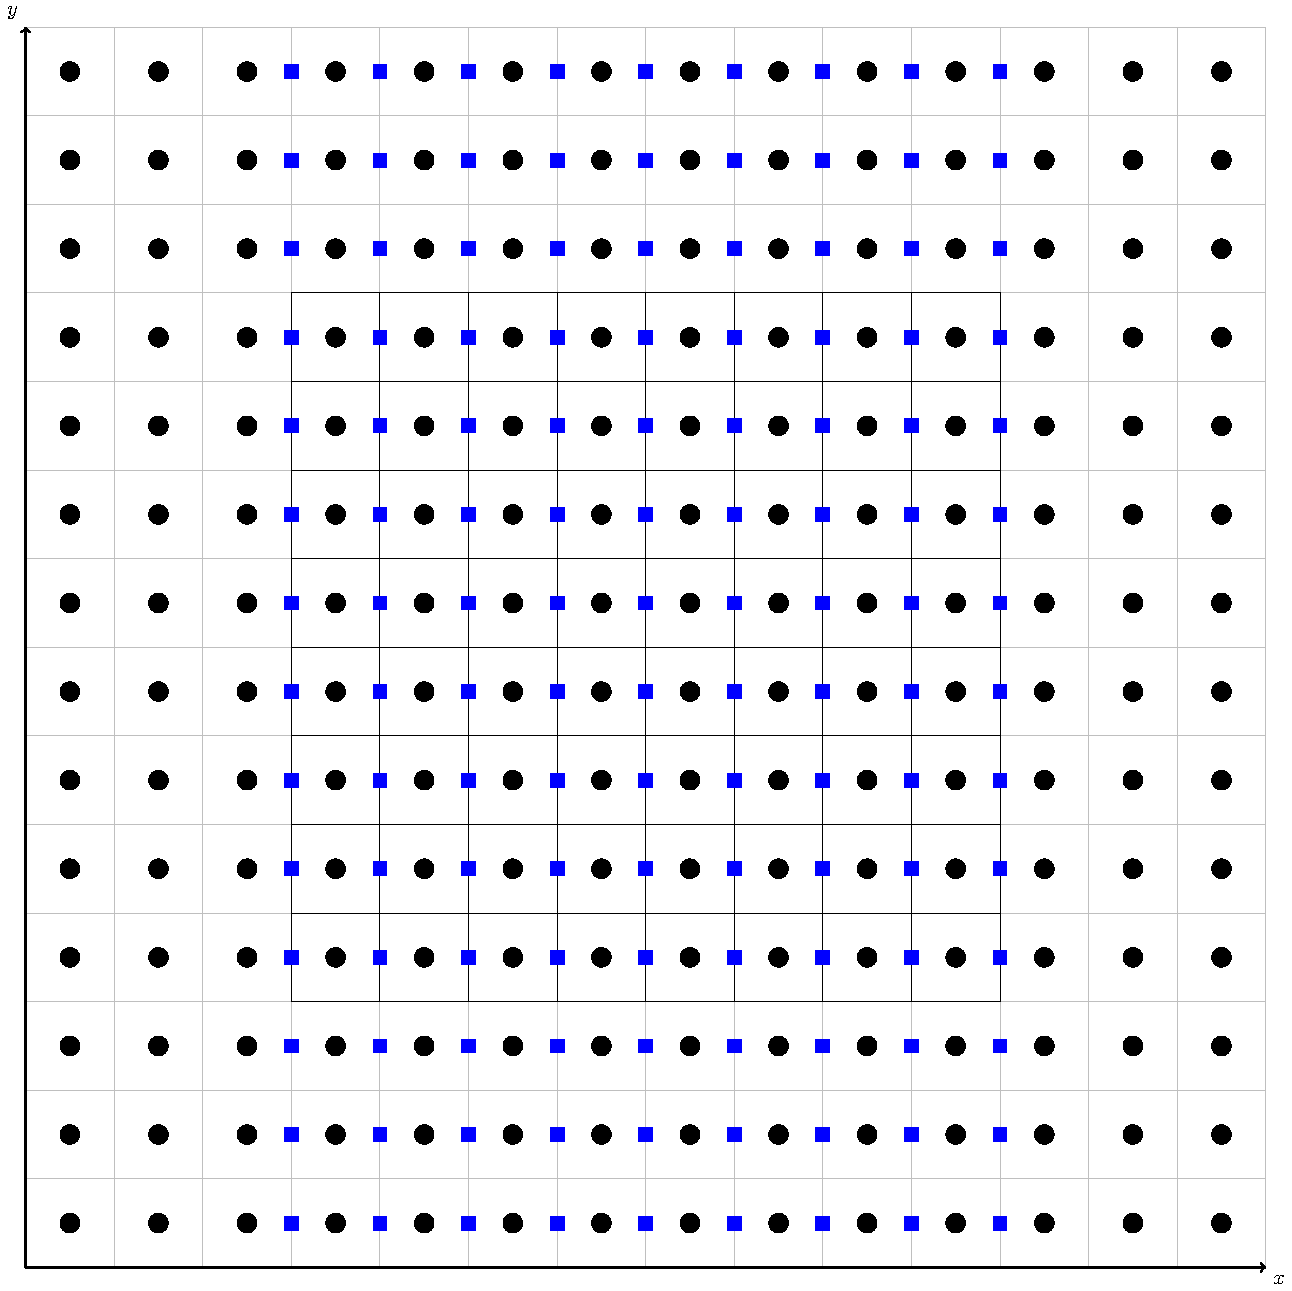
\includegraphics[width=0.95\linewidth]{2d_grid_Qx}
		\caption{$q^n$ (black circles) and $u$ at edges (blue squares). \label{lt-Qx}}
	\end{subfigure}
	\begin{subfigure}{0.3\textwidth}
		\centering
		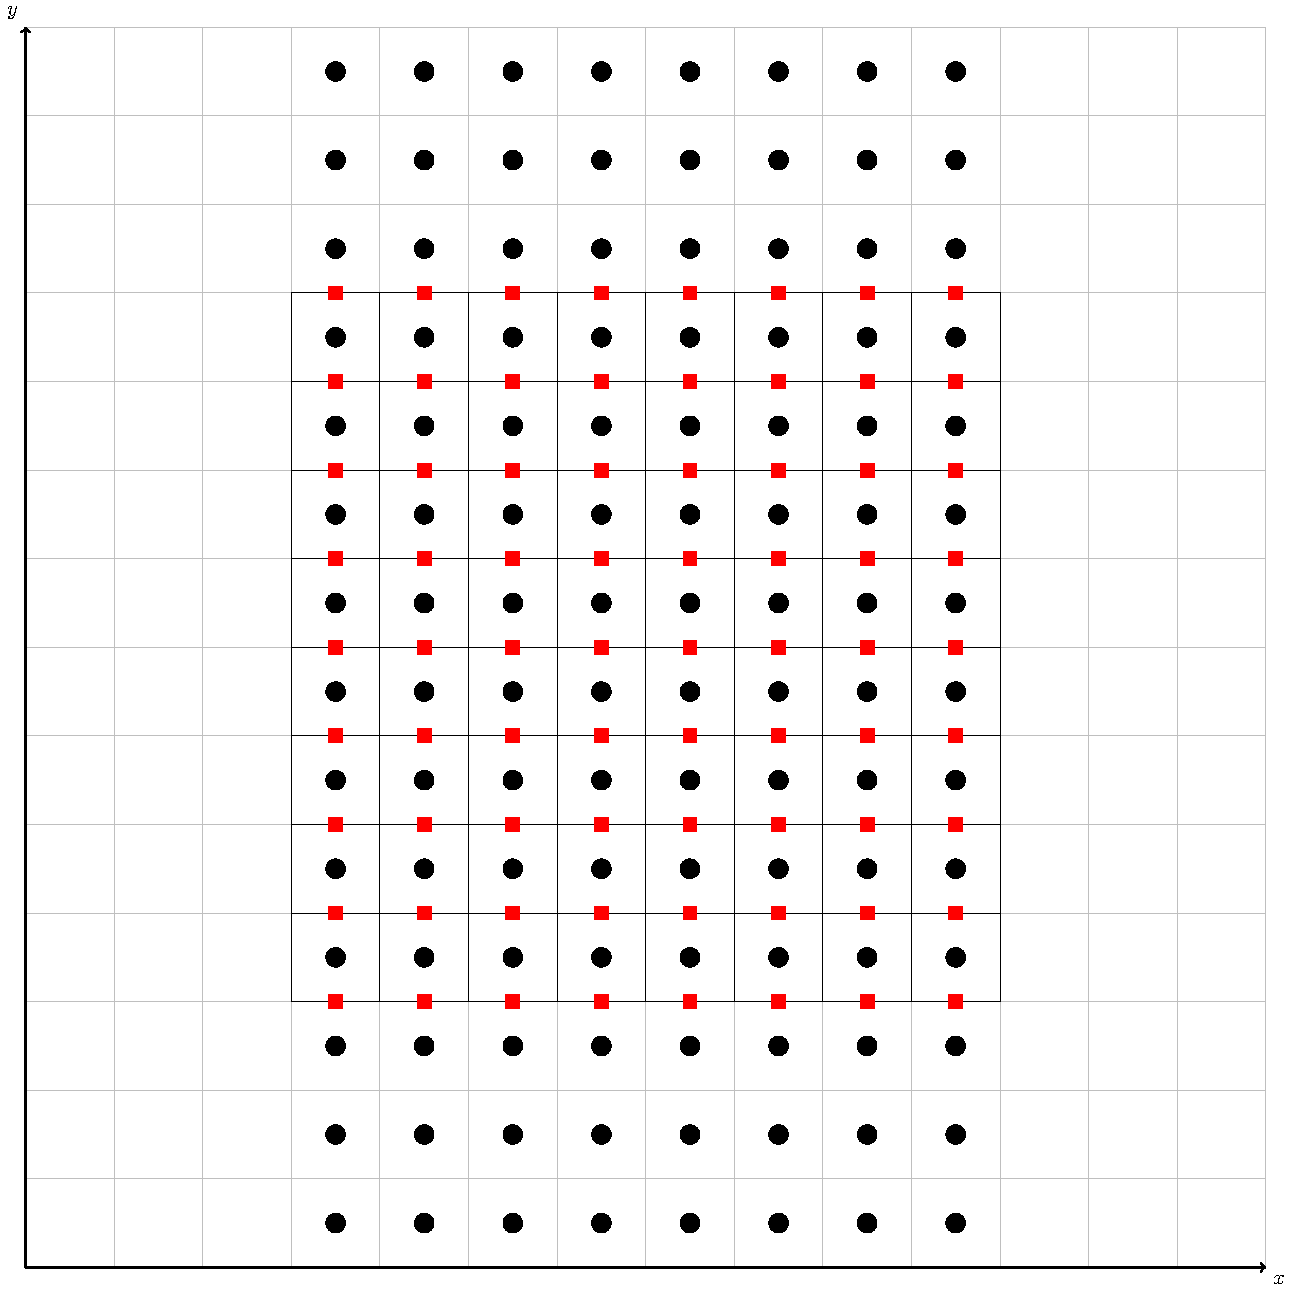
\includegraphics[width=0.95\linewidth]{2d_grid_FQ}
		\caption{$q^{x,n}$ (black circles) and $v$ at edges (red squares).\label{lt-FQx} }
	\end{subfigure}
	\begin{subfigure}{0.3\textwidth}
		\centering
		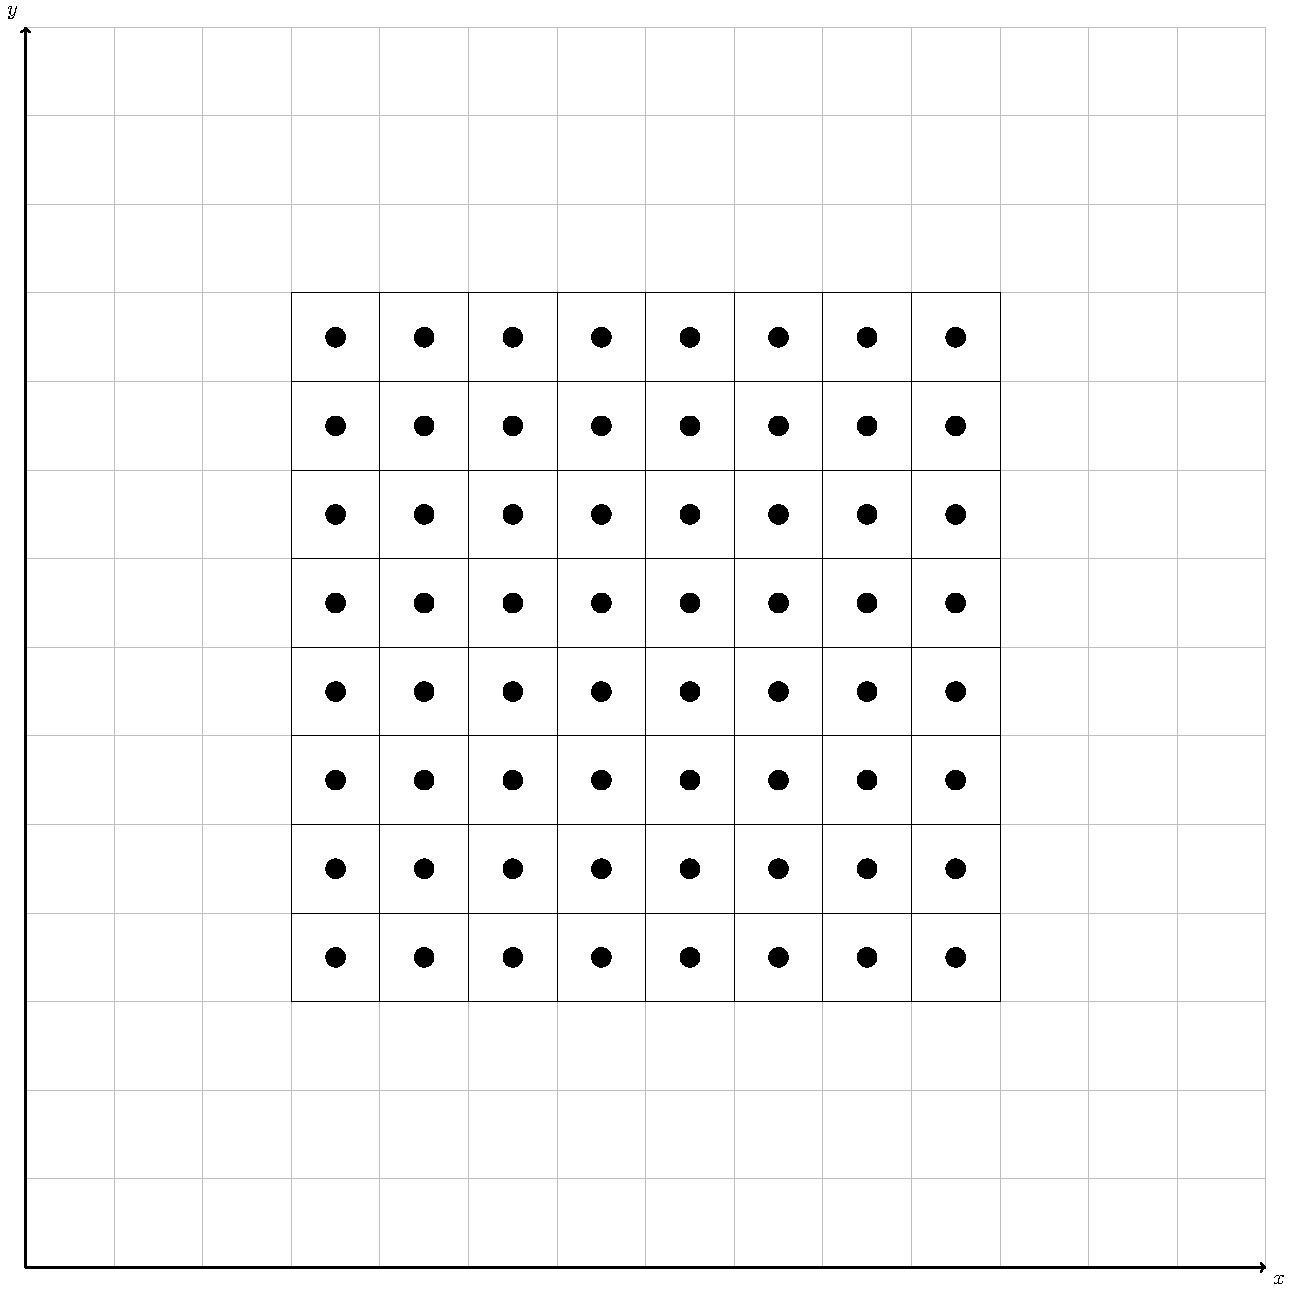
\includegraphics[width=0.95\linewidth]{2d_grid_GFQ}
		\caption{$q^{yx,n}$ (black circles) after advecting $q^{x,n}$ in $y$ direction. \label{lt-GFQx}}
	\end{subfigure}
	\caption{Illustration of the Lie-Trotter splitting on a cubed-sphere panel, where the $\mathbf{F}^M$ operator is applied in the $x$ direction (a)
	and then in the $\mathbf{G}^M$ operator in the $y$ direction.
	Interior cells are depicted using black lines,
	while ghost cells are depicted using gray lines. 
	All the winds shown are the ones used in the FV3 departure point scheme.
	If the RK2 scheme is used, an additional layer of wind ghost values should be added at each boundary in (a) and (b). \label{ltxdir}}
\end{figure}

Notice that this process may be repeated in the reverse order by solving the conservative transport equation, swapping the $x$ and $y$ directions, to obtain another solution ${q}^{xy,n}_{ij}$.
Thus the average of the solutions is considered as the final approximation:
\begin{align}
	\label{lt-scheme0}
	{q}^{n+1} = \frac{({q}^{xy,n} + {q}^{yx,n})}{2},
\end{align}
or more explicitly:
\begin{align}
	\label{lt-scheme}
	{q}^{n+1} 
	= {q}^n &+ \frac{1}{2}\mathbf{F}^M({q}^n,\tilde{c}^{M}_x) +
	\frac{1}{2}\mathbf{F}^M\bigg({q}^n + \mathbf{G}^M({q}^n, \tilde{c}^{M}_y),\tilde{c}^{M}_x\bigg)\nonumber \\
	&+\frac{1}{2}\mathbf{G}^M({q}^n,\tilde{c}^{M}_y) + 
	\frac{1}{2}\mathbf{G}^M\bigg({q}^n + \mathbf{F}^M({q}^n, \tilde{c}^{M}_x), \tilde{c}^{M}_y\bigg).
\end{align}
This scheme is an average of two Lie-Trotter splitting
and was one of the splitting schemes investigated by \cite{strang:1968}, and it is second-order accurate provided the 1D subproblems are solved with at least second-order accuracy.

As discussed by \cite{lin:1996}, when the scalar field $q^n$ is constant and the wind is divergent free, the scheme \eqref{lt-scheme} introduces a splitting error.
Aiming to eliminate the splitting error that arises in this situation, \cite{lin:1996} proposes to consider a modification of the scheme \eqref{lt-scheme} as:
\begin{align}
	\label{tr-scheme}
	{q}^{n+1}  
	= {q}^n &+ \frac{1}{2}\mathbf{F}^M({q}^n,\tilde{c}^{M}_x) +
	\frac{1}{2}\mathbf{F}^M\bigg({q}^n + \mathbf{g}^M({q}^n,  \tilde{c}^{M}_y), \tilde{c}^{M}_x\bigg) \nonumber\\
	&+\frac{1}{2}\mathbf{G}^M({q}^n, \tilde{c}^{M}_y) + 
	\frac{1}{2}\mathbf{G}^M\bigg({q}^n + \mathbf{f}^M({q}^n,  \tilde{c}^{M}_x), \tilde{c}^{M}_y\bigg),
\end{align}
where, $\mathbf{f}$ and $\mathbf{g}$ are called inner advection operators, designed to eliminate the splitting error that arises when the scalar field is constant and the wind is divergence-free.
In particular, the inner advection operators of \cite{putman:2007,harris:2016} are considered. 
Their expressions are given by:
\begin{equation}
	\mathbf{f}_{ij}^{\text{FV3}}({q}^n, \tilde{c}^{\text{FV3}}_x) = 
	-{q}_{ij}^n +
	\frac{{q}_{ij}^n + \mathbf{F}_{ij}^{\text{FV3}}({q}^n,\tilde{c}^{\text{FV3}}_x)}{1  + \mathbf{F}_{ij}^{\text{FV3}}(\mathbf{1},\tilde{c}^{\text{FV3}}_x)},
\end{equation}
where, $\mathbf{1}$ is the constant grid function equal to one.
The inner operator  $\mathbf{g}^{\text{FV3}}$ is defined similarly using $\mathbf{G}^{\text{FV3}}$.
One can easily see that the splitting error is indeed eliminate for the constant scalar field and divergence-free wind when using the FV3 scheme.
This happens because the FV3 scheme satisfies Equation  \eqref{F-operator-prop}.

The LT2 scheme does not satisfy Equation \eqref{F-operator-prop}.
Therefore, this scheme considers simply $\mathbf{f}^{\text{LT2}}=\mathbf{F}^{\text{LT2}}$ and $\mathbf{g}^{\text{LT2}}=\mathbf{G}^{\text{LT2}}$.
Despite the elimination of the splitting error for the constant scalar field and divergence free wind will no longer hold, since the 1D LT2 scheme is second-order accurate, the final LT2 scheme is expected to be second-order accurate, since it is given by Equation \eqref{lt-scheme}.
Although the 1D FV3 scheme is only first-order accurate, the elimination property of the final FV3 scheme guarantees that it behaves as second-order for divergence-free winds, as will be demonstrated in numerical simulations.

We would like to point out that both FV3 and LT2 schemes, as they use the PPM as the 1D solver, result in the final 2D schemes employing a C-grid staggering, as named by \cite{arakawa:1977}, for the wind positions (Figure \ref{cgrid}). 
The transported quantity is located at the cell centers.
Furthermore, both schemes are written in flux-form, making them adequate for preserving total mass. 
However, on the cubed-sphere, as pointed out by \cite{ross:2006,chen:2021,mouallem:2023}, the fluxes at the cube edges are computed twice, potentially leading to a mismatch that disrupts total mass conservation. 
To address this and ensure mass conservation, this work considers a simple average of the fluxes at the cube edges, following the works mentioned before.

As pointed out in Figure \ref{ltxdir}, both FV3 and LT2 schemes require C-grid contravariant wind components at ghost cells, with the LT2 scheme requiring only an extra ghost cell layer at each boundary.
These values may be obtained similarly to the interpolation process described in Section \ref{cs-ghost}, but conversions from cube to latitude-longitude coordinates (\ref{ap-wind}) are needed to avoid the cubed-sphere discontinuity. The inverse transform is performed after the interpolation is done.
This process's details are highlighted in \cite[Section 2.3]{mouallem:2023}.

To concluded this section, the transport model described by Equations \eqref{transp-rho} and \eqref{transp-phi} may be solved using the scheme from Equation \eqref{tr-scheme}, applied considering $q^n=\rho^n$ and $q^n=(\rho \phi)^n$ simultaneously.
In this framework, the tracer concentration is given by $\phi^n = \frac{(\rho \phi)^n}{\rho^n}$.

%%%%%%%%%%%%%%%%%%%%%%%%%%%%%%%%%%%%%%%%%%%%%%%%%%%%%%%%%%%%%%
\section{Numerical experiments}
\label{num-exp}
\textcolor{red}{
In this section, the goal is to present simulations of the numerical solution of the transport model, governed by Equations \eqref{transp-rho} and \eqref{transp-phi}, utilizing the FV3 and LT2 schemes. As mentioned earlier, the tracer concentration $\phi$ is advected in the transport model.}
To specify the simulation, including the initial condition for the tracer concentration $\phi_0$, the zonal wind component  denoted by $u_\lambda$, and the meridional wind component denoted by $v_\theta$, need to be defined.
The conversion from these wind components to cubed-sphere contravariant wind components (Equation \eqref{contravariant-wind}) is detailed in \ref{ap-wind}.

The initial density $\rho$ is assumed to be equal to one for all tests.
For all simulations presented here it is adopted $R= 6.371\times 10^6$ meters, equivalent to the Earth's radius. 
The final integration time is set to $T=12 \times 86400$ seconds, equivalent to 12 days.

To compute convergence, cubed-sphere grids with values of $N_k = 48 \times 2^{k}$ and time steps $\Delta t^{(k)} = \frac{\Delta t^{(0)}}{2^k}$ for $k = 0, \ldots, 4$ are considered, where the value of $\Delta t^{(0)}$ will be specified for each test case.

The $p$-norm, $p \ge 1,$ for a cubed-sphere grid function $q_{ijm}$ is defined as:
\begin{equation}
	\label{pnorm}
	\|q\|_{p}=
	\begin{cases}
		\bigg( \sum_{m=1}^{6} \sum_{i,j=1}^{N} |q_{ijm}|^p |\Omega_{ij}|\bigg)^{\frac{1}{p}} & \text{if } 1\leq p < \infty,\\
		\max_{i,j=1, \ldots, N,m=1,\ldots,6}{|q_{ijm}|} & \text{if } p=\infty.
	\end{cases}
\end{equation}
\textcolor{red}{
The relative error in the $p$-norm are computed as:
\begin{equation}
	\label{error-pnorm}
	E_p^{(k)} = \frac{\|q^{\text{REF}}-q\|_p}{\|q^{\text{REF}}\|_p},
\end{equation}
for $k=0,\ldots,4$,
where $q^{\text{REF}}$ is the reference solution.
In particular, $p=2$ (corresponding to the $L_2$ error) and $p=\infty$ (corresponding to the $L_{\infty}$ error) are considered for the tracer concentration, where $q=\phi$.
The order of convergence is computed as
\begin{equation}
\text{order} = {\ln{\bigg(\frac{E_4}{E_{3}}\bigg)}}
\frac{1}{\ln{2}}.
\end{equation}}

\subsection{Rotated zonal wind experiments}
In this section, the following rotated zonal wind field based on \cite{will:1992} is considered:
\begin{align}
	\label{zonal-wind}
	\begin{cases}
		u_\lambda(\lambda,\theta,t) = u_0(\cos(\theta)\cos(\alpha) + \sin(\theta)\cos(\lambda)\sin(\alpha)),\\
		v_\theta(\lambda,\theta,t) = -u_0\sin(\lambda)\sin(\alpha),
	\end{cases}
\end{align}
where $\lambda \in [-\pi,\pi]$ represents longitude and $\theta \in [-\frac{\pi}{2},\frac{\pi}{2}]$ represents latitude. 
It is easy to see that the wind is divergence free.
The parameter $\alpha$ is the rotation angle. Following \cite{putman:2007}, the rotation angle is set as $\alpha=\frac{\pi}{4}$ so that the wind is oriented with the cube corners. 
Finally, the parameter $u_0$ is defined as $u_0 = \frac{2\pi R}{T}$.
With this choice, the simulation period is 12 days. The solution should converge to the initial condition after this period, enabling us to compute the final error.
Therefore, the temporal evolution of the error may be analyzed.
For an expression of the exact solution in this case and a general initial condition, refer to \cite[Theorem 5.1, p. 155]{brachet:2018}.
The time-step for $N=48$ is given by $\Delta t^{(0)} = 3600$ seconds, leading to a CFL number of approximately 0.95. 

Initially, the initial condition is given by the following Gaussian hill at a cube corner:
\begin{align}
\phi_0(P) = \exp(-b_0((p_x-p_x^0)^2+ (p_y-p_y^0)^2 + (p_z-p_z^0)^2)),
\end{align}
for $P \in \mathbb{S}_R^2$.
It is considered $p_x^0=p_y^0=p_z^0=\frac{1}{\sqrt{3}}$ and
$b_0=10$.
Therefore, the Gaussian hill is indeed centered at a cube corner.
Hence, in this test, the Gaussian hill is translated over 4 cube corners, enabling the assessment of the schemes' sensitivity to these corners.
\begin{figure}[!htb]
	\centering
	\begin{subfigure}{0.45\textwidth}
	\centering
	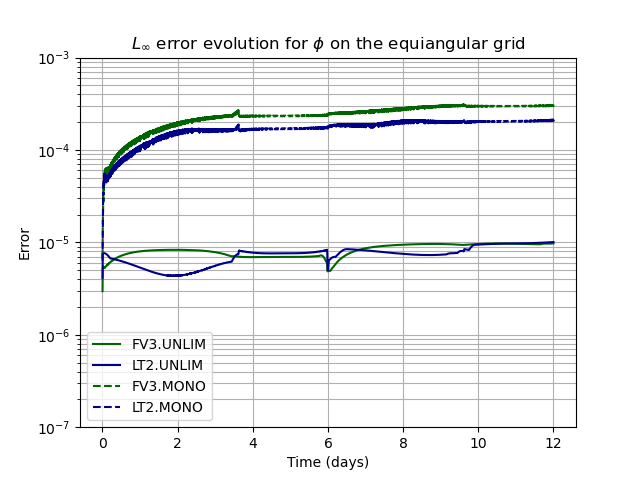
\includegraphics[width=1.1\linewidth]{tc-3_C768_linf_errors_equiangular}
	\caption{Equiangular grid\label{GH-equiangular-evol}}
    \end{subfigure}
	\begin{subfigure}{0.45\textwidth}
		\centering
		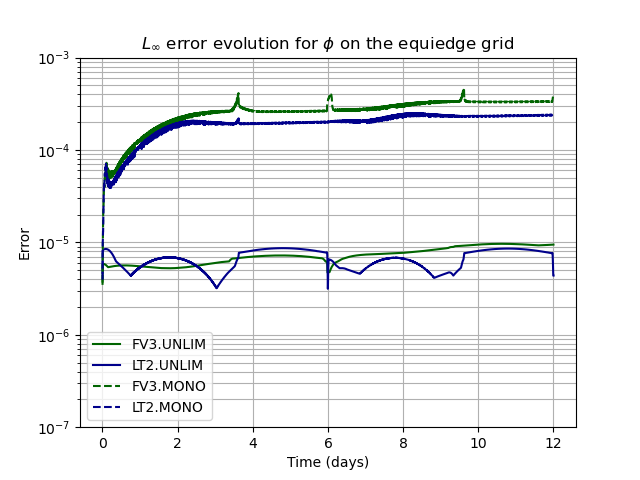
\includegraphics[width=1.1\linewidth]{tc-3_C768_linf_errors_equiedge}
		\caption{Equi-edge grid\label{GH-equiedge-evol}}
	\end{subfigure}
	\caption{
The $L_{\infty}$ error evolution for the tracer concentration $\phi$ in the transport model with a Gaussian hill as the initial condition using the rotated zonal wind is illustrated on the equiangular  (a) and on the equi-edge (b) grids for 12 days and $N=768$.
Blue lines indicate the use of the LT2 scheme, while green lines represent the FV3 scheme.
Solid lines represent the results with the unlimited PPM (UNLIM) scheme, whereas dashed lines represent the results with the monotonic (MONO).
\label{GH-linf-evol}}
\end{figure}

In fact, Figure \ref{GH-linf-evol} shows how the error evolves with time over 12 days in the $L_{\infty}$ norm for $N=768$ for both equi-edge and equiangular grids.
This Figure use green lines to represent the FV3 scheme and blue lines to represent the LT2 scheme.
Dashed lines represent the monotonic while solid lines represent the unlimited PPM.
From Figure \ref{GH-linf-evol} some small spikes are observed in the $L_{\infty}$ error
on the equi-edge grid (Figure \ref{GH-equiedge-evol}) when using both schemes with MONO, which is less pronounced on the equiangular grid (Figure \ref{GH-equiangular-evol}).
On the equi-edge grid (Figure \ref{GH-equiedge-evol}), the spikes are less pronounced for the LT2 scheme.

Figure \ref{GH-corner} illustrates the final error at a cube corner for the equi-edge grid. Similar results are obtained for the equiangular grid, but are omitted here.
It is clear that the errors for the FV3 scheme are larger at the corners (Figure \ref{GH-FV3-corner}) compared to the corner errors of the LT2 scheme (Figure \ref{GH-LT2-corner}), being almost 1.6 times bigger.

\begin{figure}[!htb]
	\centering
	\begin{subfigure}{0.45\textwidth}
		\centering
		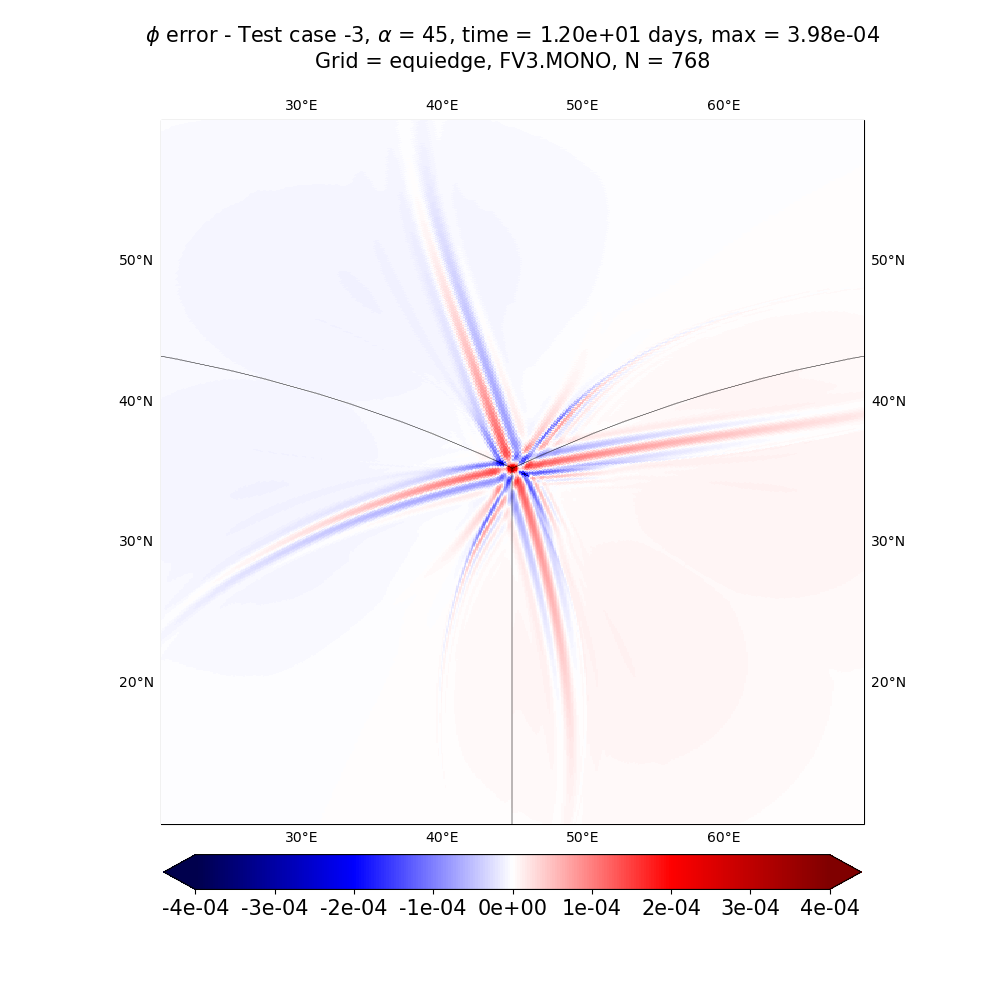
\includegraphics[width=1.1\linewidth]{h_error_tc-3_t12_alpha45_C768_g0_dg2_adv1_hord8_mf1_tf12}
		\caption{FV3 - max = $3.98 \times 10^{-4}$.\label{GH-FV3-corner}}
	\end{subfigure}
	\begin{subfigure}{0.45\textwidth}
		\centering
		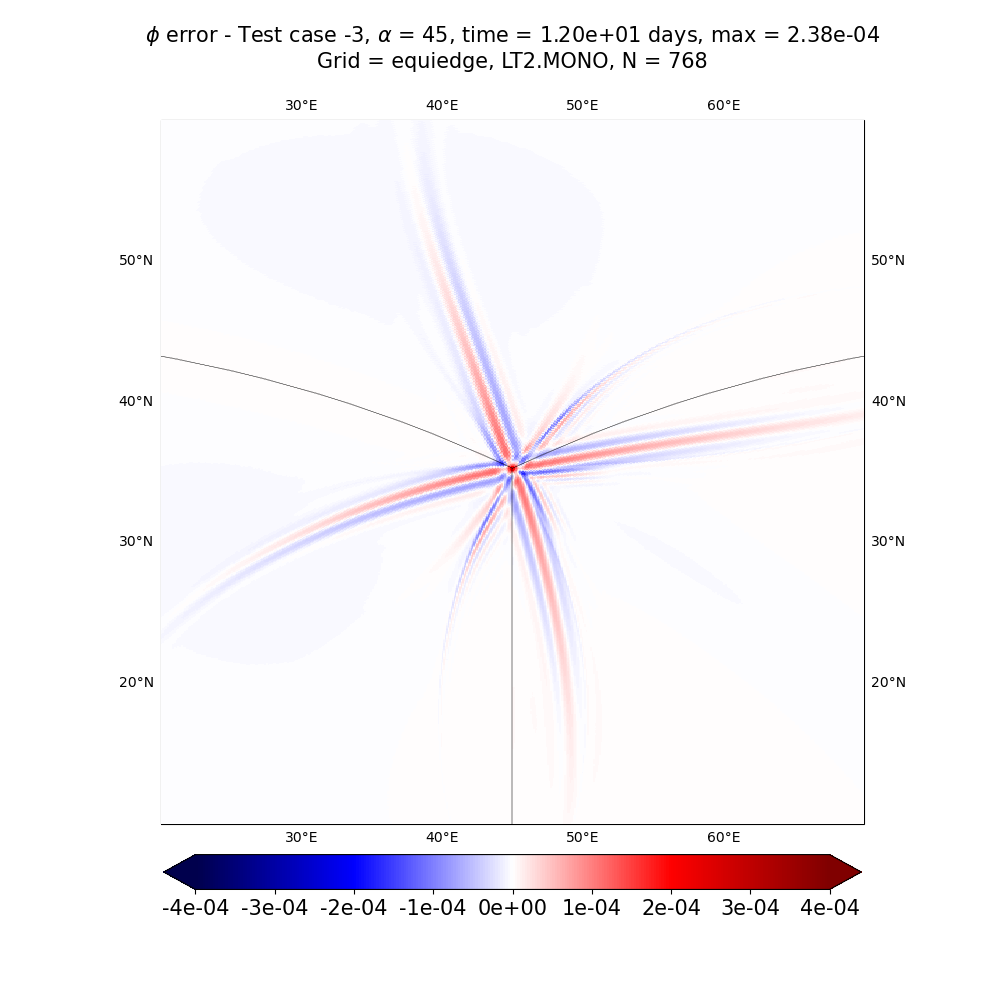
\includegraphics[width=1.1\linewidth]{h_error_tc-3_t12_alpha45_C768_g0_dg2_adv2_hord8_mf1_tf12}
		\caption{LT2 - max = $2.38 \times 10^{-4}$.\label{GH-LT2-corner}}
	\end{subfigure}
	\caption{Errors at a cube corner after 12 days of the tracer concentration $\phi$ in the transport model for the test case using the Gaussian hill and the rotated zonal wind, employing the monotonic scheme (MONO) with FV3 (a) and LT2 schemes (b) on the equi-edge grid with $N=768$. 
	\label{GH-corner}}
\end{figure}


\begin{figure}[!htb]
	\centering
	\begin{subfigure}{0.45\textwidth}
	\centering
	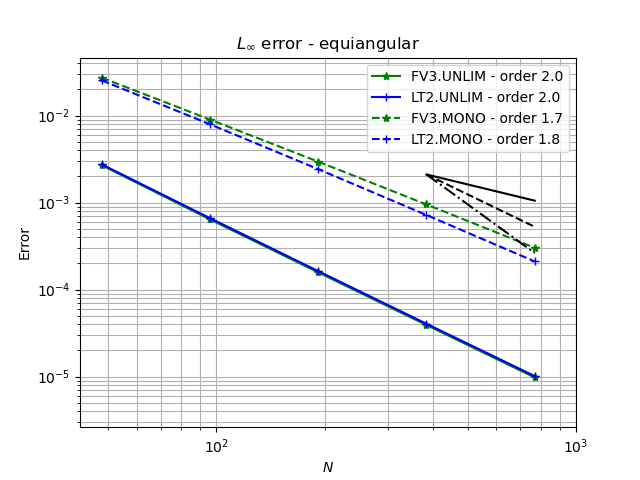
\includegraphics[width=1.1\linewidth]{linferror_tc-3_alpha45.equiangular}
	\caption{Equiangular grid\label{GH-equiangular-linf}}
    \end{subfigure}
	\begin{subfigure}{0.45\textwidth}
		\centering
		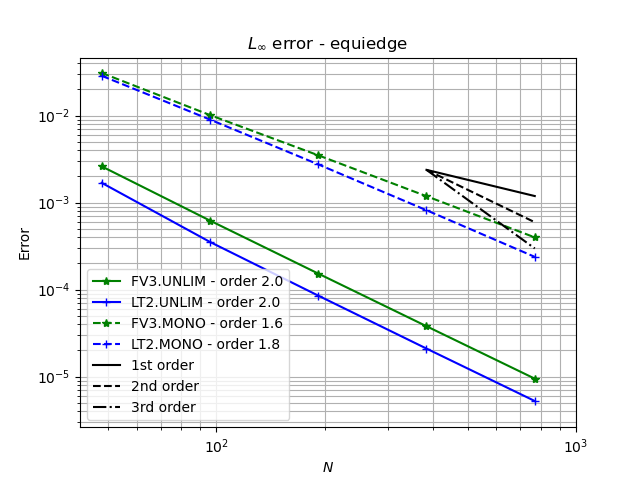
\includegraphics[width=1.1\linewidth]{linferror_tc-3_alpha45.equiedge}
		\caption{Equi-edge grid\label{GH-equiedge-linf}}
	\end{subfigure}
	\caption{
	$L_{\infty}$ error convergence for the tracer concentration $\phi$ in the transport model using the Gaussian hill  as the initial condition and  the rotated zonal wind on the equiangular (a)
	and on the equi-edge  (b) grids after 12 days.
	Blue lines indicate the use of the LT2 scheme, while green lines represent the FV3 scheme.
	Solid lines represent the results with the unlimited PPM (UNLIM) scheme, whereas dashed lines represent the results with the monotonic PPM (MONO).
	\label{GH-linf}}
\end{figure}

\begin{figure}[!htb]
	\centering
	\begin{subfigure}{0.45\textwidth}
	\centering
	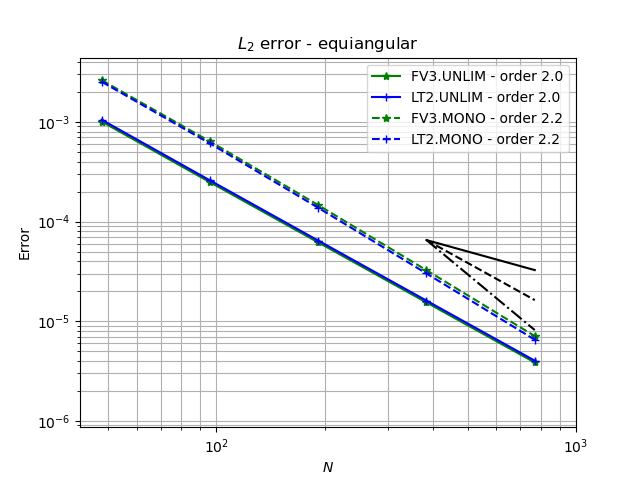
\includegraphics[width=1.1\linewidth]{l2error_tc-3_alpha45.equiangular}
	\caption{Equiangular grid\label{GH-equiangular-2}}
    \end{subfigure}
	\begin{subfigure}{0.45\textwidth}
		\centering
		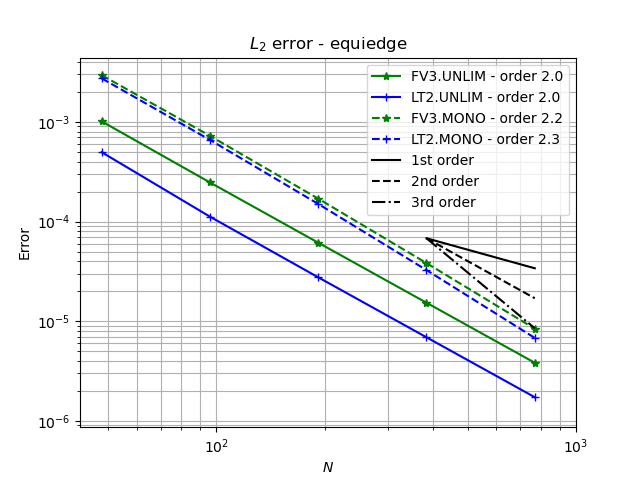
\includegraphics[width=1.1\linewidth]{l2error_tc-3_alpha45.equiedge}
		\caption{Equi-edge grid\label{GH-equiedge-l2}}
	\end{subfigure}
	\caption{As Figure \ref{GH-linf} but using $L_2$ norm.
		\label{GH-l2}}
\end{figure}
Finally, Figures \ref{GH-linf} and \ref{GH-l2} show the error convergence in $L_{\infty}$ and $L_{2}$ norms.
It can be observed that all schemes with the unlimited PPM (UNLIM) achieve second-order accuracy as expected.
However, for MONO, the order is reduced, which is also expected.
Additionally, it is observed that MONO with LT2 has smaller errors when comparing the blue dashed lines with the green dashed lines, 
for both $L_{\infty}$ and $L_{2}$ norms on both equiangular (a) and the equi-edge (b) grid, indicating that LT2 is slightly more accurate.
In general, the errors of the equi-edge are slightly smaller than those of equiangular.

\begin{figure}[!htb]
	\centering
	\begin{subfigure}{0.45\textwidth}
		\centering
		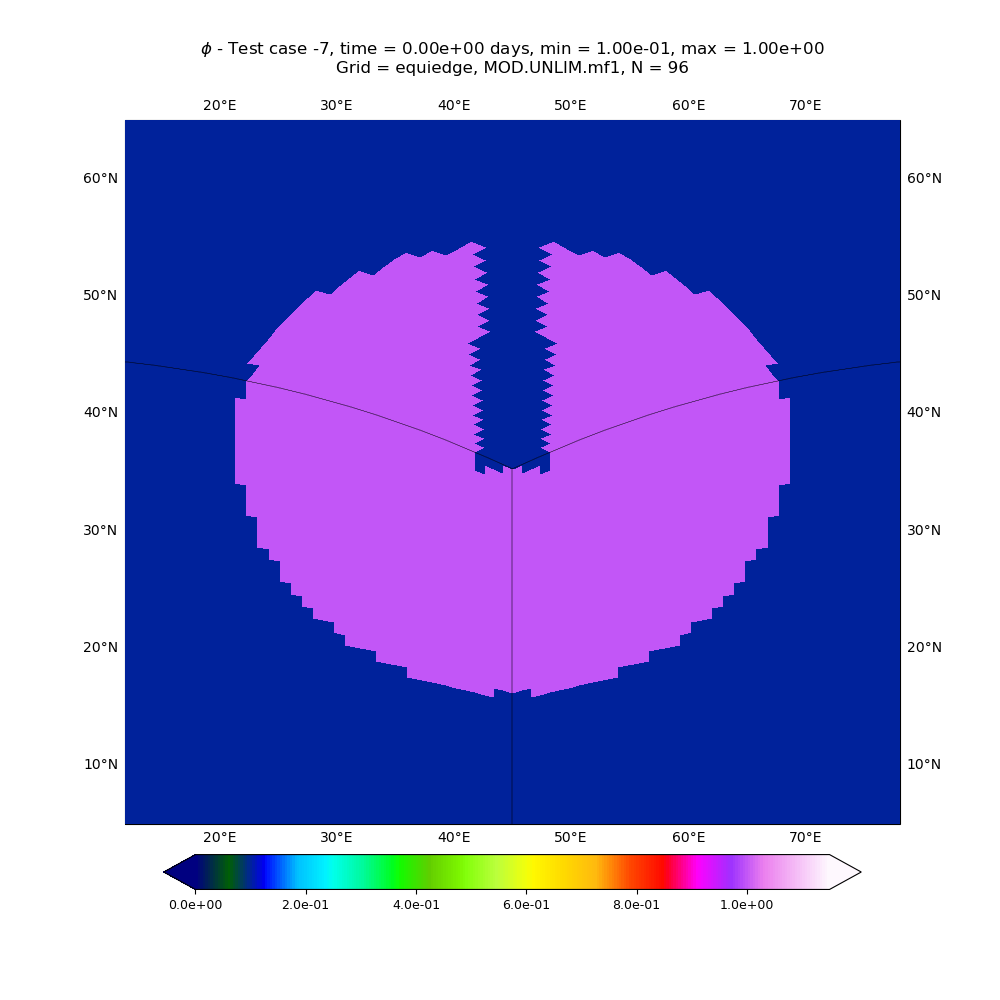
\includegraphics[width=1.1\linewidth]{h_tc-7_t0_alpha45_C96_g0_dg2_adv2_hord0_mf1_tf12}
		\caption{Exact solution\label{CY-IC}}
	\end{subfigure}
	\begin{subfigure}{0.45\textwidth}
		\centering
		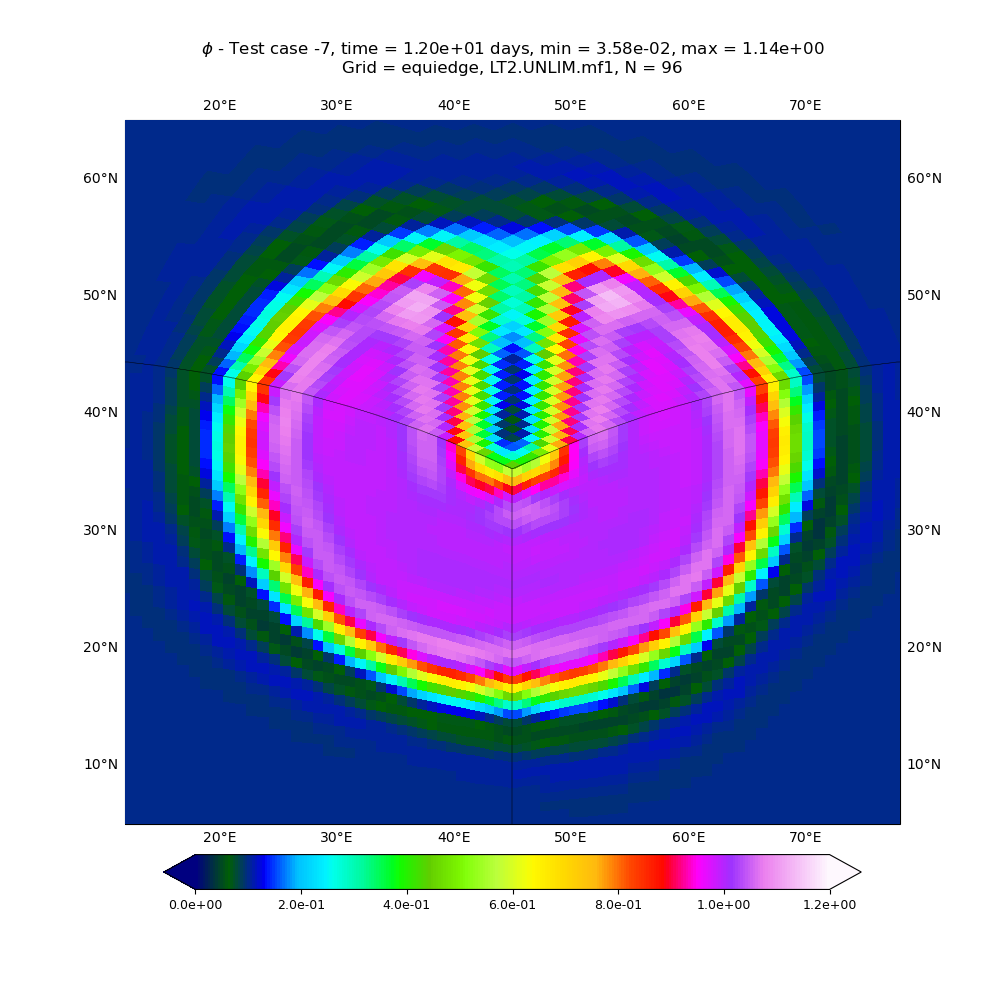
\includegraphics[width=1.1\linewidth]{h_tc-7_t12_alpha45_C96_g0_dg2_adv2_hord0_mf1_tf12}
		\caption{LT2-UNLIM\label{CY-LT2-UNLIM-corner}}
	\end{subfigure}
	
	\begin{subfigure}{0.45\textwidth}
		\centering
		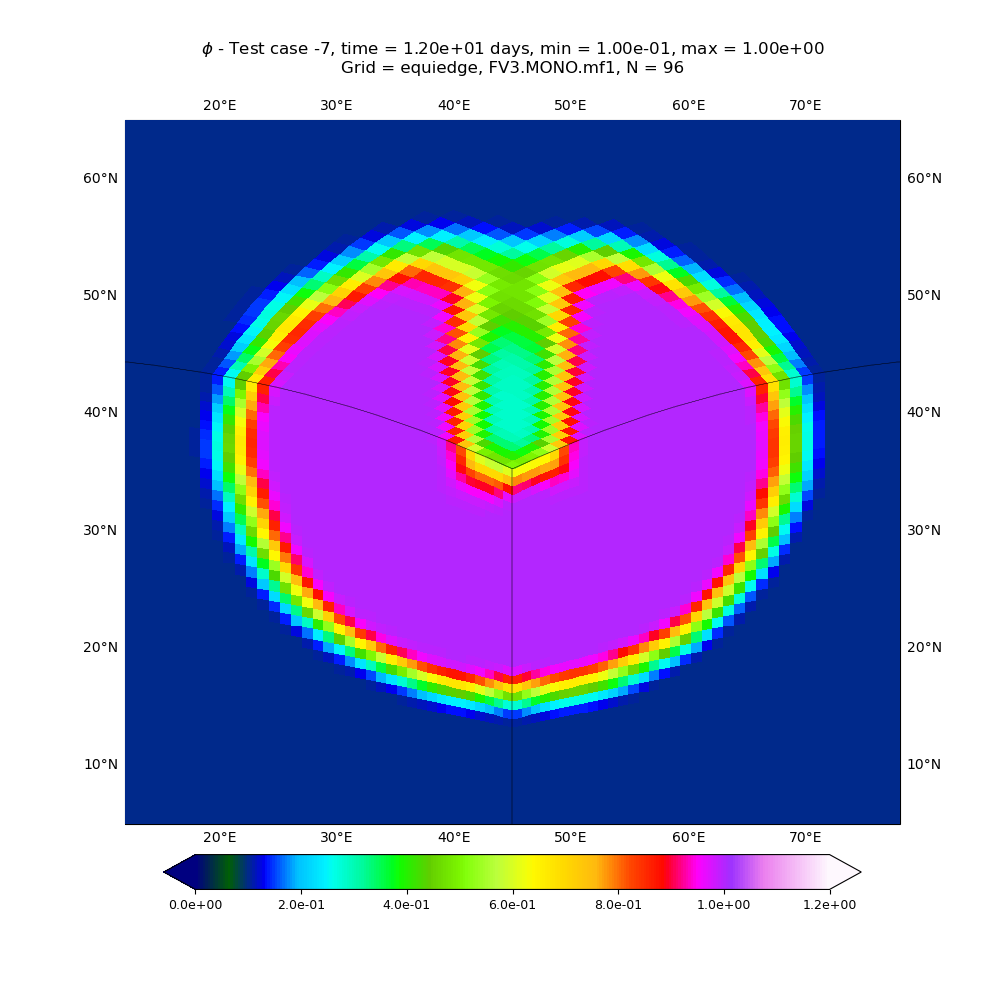
\includegraphics[width=1.1\linewidth]{h_tc-7_t12_alpha45_C96_g0_dg2_adv1_hord8_mf1_tf12}
		\caption{FV3-MONO\label{CY-FV3-MONO-corner}}
	\end{subfigure}
	\begin{subfigure}{0.45\textwidth}
		\centering
		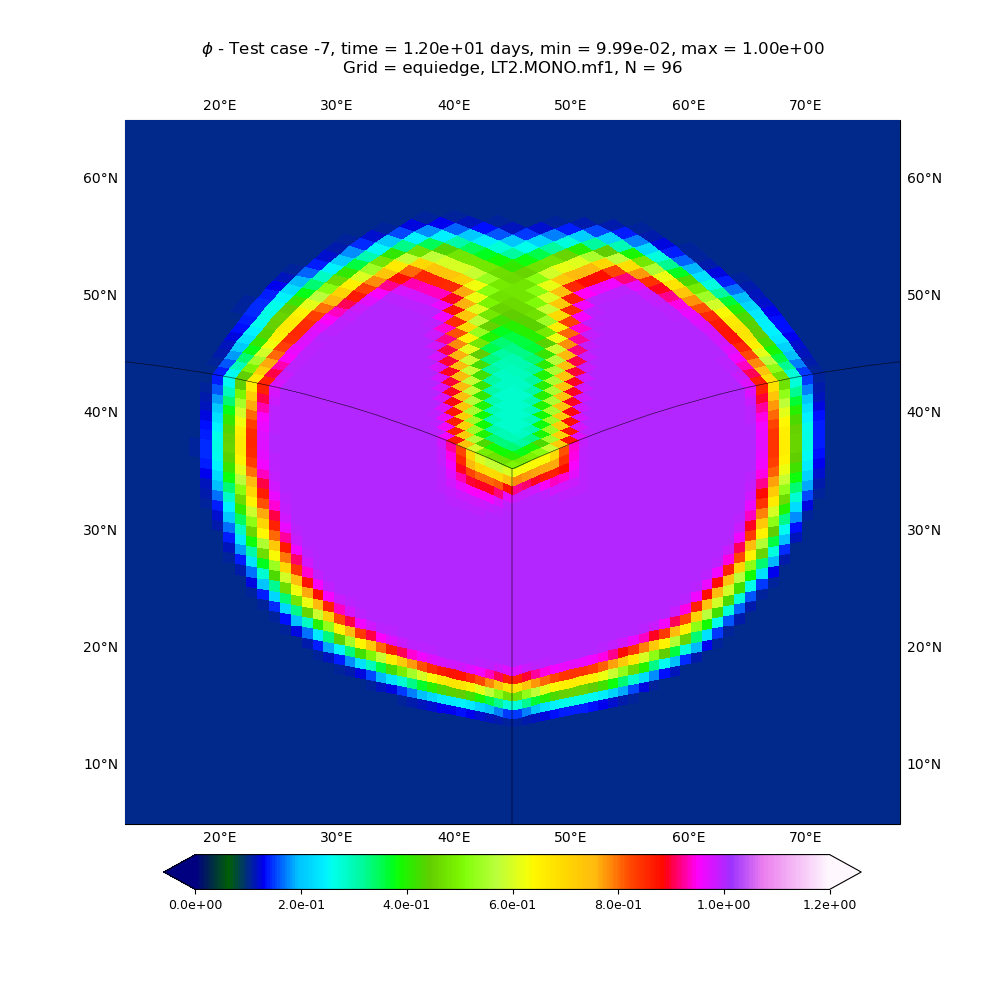
\includegraphics[width=1.1\linewidth]{h_tc-7_t12_alpha45_C96_g0_dg2_adv2_hord8_mf1_tf12}
		\caption{LT2-MONO\label{CY-LT2-MONO-corner}}
	\end{subfigure}
	\caption{Advection of a cylinder at corner, representing the tracer concentration $\phi$, with $N= 96$ after 12 days for the schemes FV3-MONO (a), LT2-MONO (b), LT2-UNLIM (c) at the equi-edge grid and the exact solution (d).}
	\label{CY-corner}
\end{figure}
To assess the difference between the UNLIM and MONO schemes for both FV3 and LT2 schemes, the slotted cylinder from \cite{nair:2010} centered a cube corner is considered.
To define the slotted cylinder, it is introduced
\begin{equation}
	r(\lambda, \theta)=2R \arcsin{\bigg(
		\sqrt{\sin^2{\bigg(\frac{\theta-\theta_0}{2}\bigg)} + \cos{\theta}\cos{\theta_0}\cos^2{\bigg(\frac{\lambda-\lambda_0}{2}\bigg)}}\bigg)},
\end{equation}
where $r$ is the geodesic distance from $(\lambda, \theta)$ to a cube corner fixed point  $(\lambda_0, \theta_0)$ with 
$\lambda_0 =\frac{\pi}{4}$, $\theta_0= \frac{\pi}{2}-\arccos{\big(\frac{1}{\sqrt{3}}\big)}$.
The slotted cylinder is defined as:
\begin{align}
	\label{slotted-cylinder}
	\phi(\lambda,\theta) =
	\begin{cases}
		0.1, \quad \text{if} \quad r(\lambda,\theta) > r_0,\\
		0.1, \quad \text{if} \quad r(\lambda,\theta) \le r_0, \quad
		|\lambda-\lambda_0| \ge 0.05, \quad \theta\ge\theta_0,\\
		1, \quad \text{otherwise},\\
	\end{cases}
\end{align}
where $r_0=\frac{R}{3}$.

The slotted cylinder is depicted in Figure \ref{CY-IC}.
The goal is to test MONO's ability to remove numerical oscillations, which create new extrema, in the case of advecting a cylinder.
Similar to the Gaussian hill case, the cylinder is translated through 4 cube corners in this test.

Figure \ref{CY-corner} presents the results for the MONO  scheme with both FV3 (Figure \ref{CY-FV3-MONO-corner}) and LT2 (Figure \ref{CY-LT2-MONO-corner}) schemes on the equi-edge grid with $N=96$.
Result for UNLIM with LT2 are show in Figure \ref{CY-LT2-UNLIM-corner}.
Similar results with the FV3 scheme for UNLIM are obtained and omitted here.
The initial cylinder is depicted in Figure \ref{CY-IC}.
It is observed that the MONO scheme effectively removes the oscillations present in the UNLIM results.
Similar results for the equiangular grid are obtained and omitted here.

\subsection{Flow deformation through a divergence free wind}
The divergence free deformational test case from \cite{nair:2010} is considered, where the time-dependent winds are given by
\begin{align}
	\label{ndiv-nair-wind}
	\begin{cases}
		u_\lambda(\lambda,\theta,t) =u_0\sin^2(\lambda_p)\sin(2\theta)\cos(\frac{\pi t}{T})+u_0\cos\theta,\\
		v_\theta(\lambda,\theta,t) = u_0\sin(2\lambda_p)\cos(\theta)\cos(\frac{\pi t}{T}),
	\end{cases}
\end{align}
where $\lambda_p=\lambda-\frac{2\pi t}{T}$ and $u_0 = \frac{2\pi R}{T}$. As pointed out in \cite{nair:2010}, a zonal background is added in $u_\lambda$, namely $u_0\cos\theta$, to avoid error cancellations.
The time-step for $N=48$ is adopted as $\Delta t^{(0)} = 1600$ seconds, leading to a CFL number of approximately 0.73.

As the initial condition, two Gaussian hills are considered, each one centered on a cube-edge. Specifically,
\begin{align}
\label{ndiv-nair-ic}
\phi_0(P) = 
&\exp(-b_0[(p_x-p_x^0)^2+ (p_y-p_y^0)^2 + (p_z-p_z^0)^2]) + \nonumber \\ 
&\exp(-b_0[(p_x-p_x^1)^2+ (p_y-p_y^1)^2 + (p_z-p_z^1)^2]),
\end{align}
for $P \in \mathbb{S}_R^2$.
Here $(p_x^0,p_y^0,p_z^0)$ and $(p_x^1,p_y^1,p_z^1)$ are the $\mathbb{R}^3$ coordinates of the latitude-longitude points
$(\lambda_1,\theta_1) = (-\frac{\pi}{4},0)$ and
$(\lambda_2,\theta_2) = ( \frac{\pi}{4},0)$, respectively.
The parameter $b_0$ is set as $b_0=5$.

\begin{figure}[!htb]
	\centering
	\begin{subfigure}{0.45\textwidth}
		\centering
		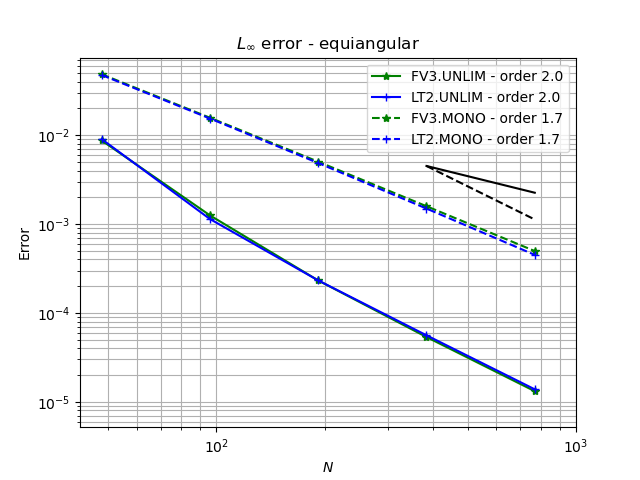
\includegraphics[width=1.1\linewidth]{linferror_tc-5_alpha0.equiangular}
		\caption{Equiangular grid\label{ndivnair-equiangular-linf}}
	\end{subfigure}
	\begin{subfigure}{0.45\textwidth}
	\centering
	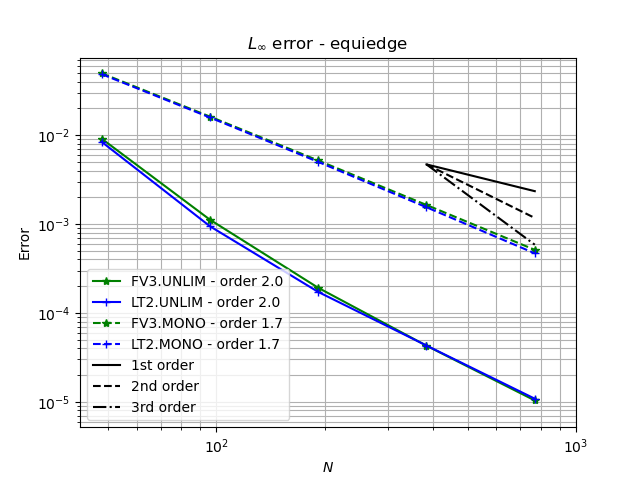
\includegraphics[width=1.1\linewidth]{linferror_tc-5_alpha0.equiedge}
	\caption{Equi-edge grid\label{ndivnair-equiedge-linf}}
    \end{subfigure}
	\caption{
		$L_{\infty}$ error convergence for the tracer concentration $\phi$ in the transport model using the two Gaussian hills  as the initial condition and  the divergence free deformational wind on equiangular (a)
and equi-edge (b) grids  after 12 days.
Blue lines indicate the use of the LT2 scheme, while green lines represent the FV3 scheme.
Solid lines represent the results with the unlimited PPM (UNLIM) scheme, whereas dashed lines represent the results with the monotonic PPM (MONO).
		\label{ndivnair-linf}}
\end{figure}

\begin{figure}[!htb]
	\centering
	\begin{subfigure}{0.45\textwidth}
		\centering
		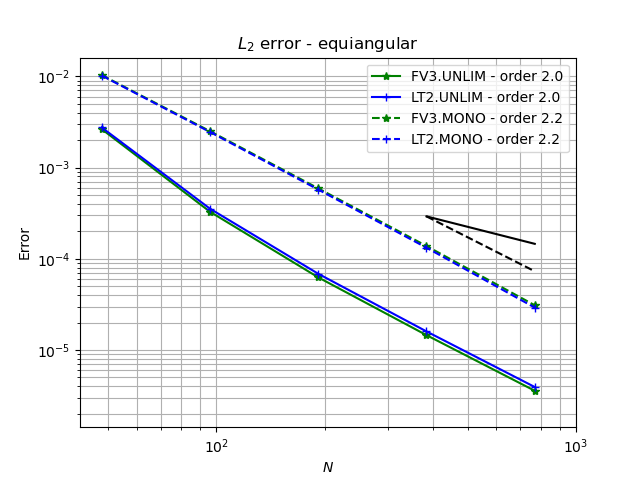
\includegraphics[width=1.1\linewidth]{l2error_tc-5_alpha0.equiangular}
		\caption{Equiangular grid\label{ndivnair-equiangular-2}}
	\end{subfigure}
	\begin{subfigure}{0.45\textwidth}
	\centering
	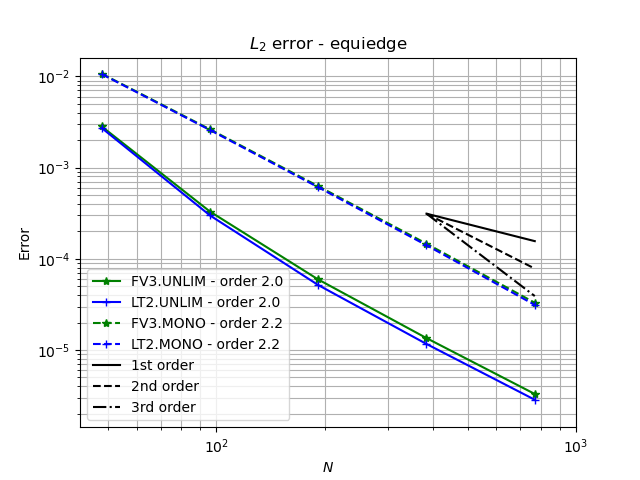
\includegraphics[width=1.1\linewidth]{l2error_tc-5_alpha0.equiedge}
	\caption{Equi-edge grid\label{ndivnair-equiedge-l2}}
    \end{subfigure}
	\caption{As Figure \ref{ndivnair-linf} but using $L_2$ norm.
		\label{ndivnair-l2}}
\end{figure}
This test deforms the Gaussian hills, without creating new extrema on the fluid density since the wind is divergence free, and the final solution is equal to the initial condition. 
Figures illustrating this process are available in \cite{nair:2010}.

Figures \ref{ndivnair-linf} and \ref{ndivnair-l2} show the error convergence in $L_{\infty}$ and $L_{2}$ norms for the  tracer concentration $\phi$.
Similar to the previous test case, it is observed that all schemes with UNLIM achieve second-order accuracy, while for MONO, the order is reduced.
Once more, the errors of the equi-edge grid are slightly smaller than those from the equiangular grid.

\subsection{Flow deformation through a divergent wind}
Finally, the divergent deformational test case from \cite{nair:2010} is considered, where the time-dependent winds are given by
\begin{align}
	\label{div-nair-wind}
	\begin{cases}
		u_\lambda(\lambda,\theta,t) =-u_0\sin^2(\frac{\lambda+\pi}{2})\sin(2\theta)\cos^2(\theta)\cos(\frac{\pi t}{T}),\\
		v_\theta(\lambda,\theta,t) = \frac{u_0}{2}\sin(\lambda+\pi)\cos^3(\theta)\cos(\frac{\pi t}{T}),
	\end{cases}
\end{align}
where $u_0 = \frac{\pi R}{2T}$.
The time-step for $N=48$ is adopted as $\Delta t^{(0)} = 6400$ seconds, leading to a CFL number of approximately 0.91. 
The initial conditions are again the two Gaussian hill (Equation \eqref{ndiv-nair-ic}).
Unlikely the previous tests, this test introduces a divergent wind.
This test deforms the Gaussian hills, creating new extrema for the tracer density $\rho \phi$, and the final solution is equal to the initial condition. 
Figures illustrating this process are available in \cite{nair:2010}.

\begin{figure}[!htb]
	\centering
	\begin{subfigure}{0.45\textwidth}
		\centering
		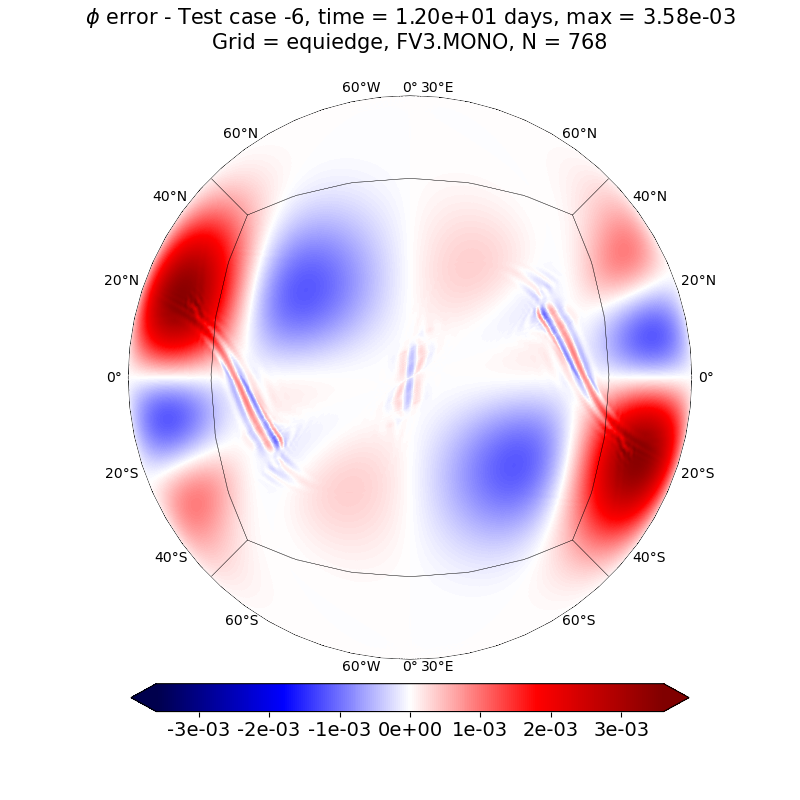
\includegraphics[width=1.1\linewidth]{h_error_tc-6_t12_alpha0_C768_g0_dg2_adv1_hord8_mf1_tf12}
		\caption{FV3 scheme - max=$3.58 \times 10^{-3}$. \label{divnair-error-FV3}}
	\end{subfigure}
	\begin{subfigure}{0.45\textwidth}
		\centering
		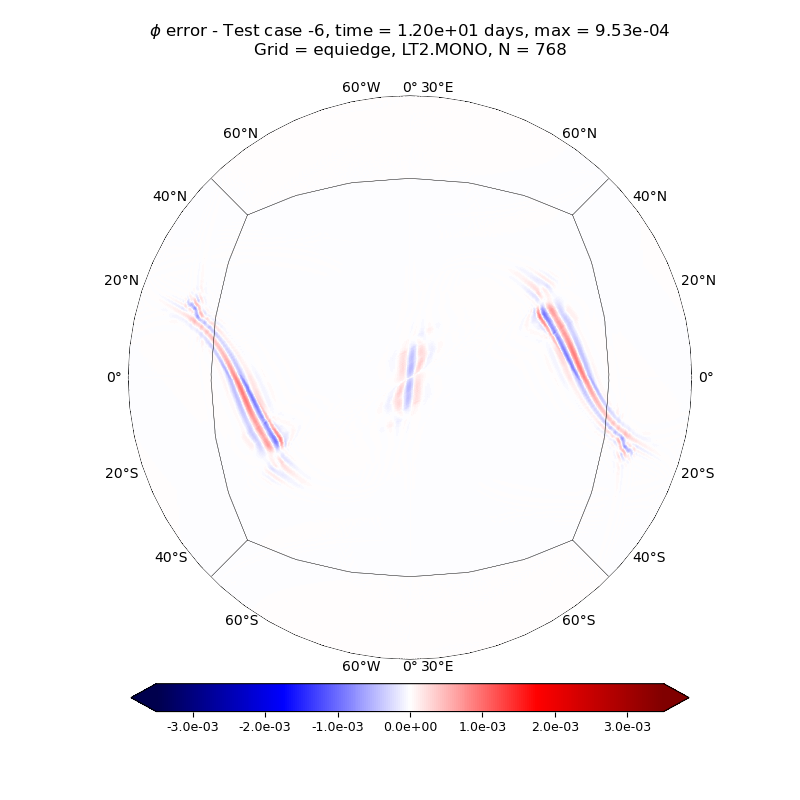
\includegraphics[width=1.1\linewidth]{h_error_tc-6_t12_alpha0_C768_g0_dg2_adv2_hord8_mf1_tf12}
		\caption{LT2 scheme - max=$9.53 \times 10^{-4}$.\label{divnair-error-LT2}}
	\end{subfigure}
	\caption{
		Transport experiment errors for the tracer concentration $\phi$ using the two Gaussian hills  and  the divergent wind  after 12 days, using the monotonic scheme (MONO)
		with FV3 (a) and LT2 (b) schemes on the equi-edge grid  with $N=768$.
		\label{divnair-error}}
\end{figure}

Figures \ref{divnair-error-FV3} and \ref{divnair-error-LT2} display the final error of the tracer concentration $\phi$ at a cube face for the equi-edge grid using the MONO scheme.
Similar results on the equiangular grid are obtained and not shown here.
The errors for the FV3 scheme are observed to be much larger, with the maximum error being four times that of the LT2 scheme. 
Significant errors are present in many cells for FV3, whereas the errors in the LT2 scheme are smaller and concentrated in some ripples.

\begin{figure}[!htb]
	\centering
	\begin{subfigure}{0.45\textwidth}
	\centering
	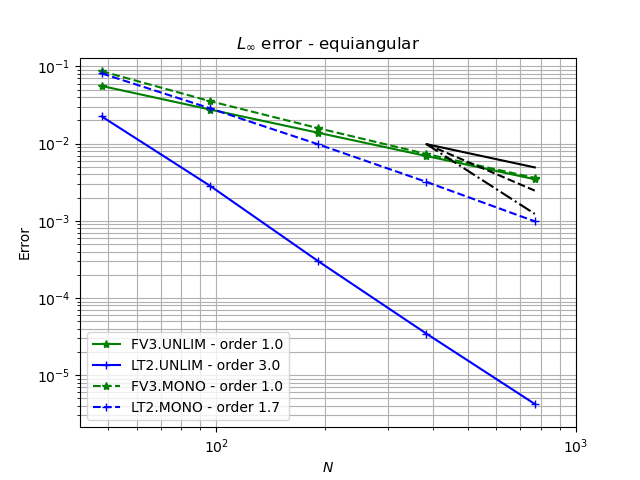
\includegraphics[width=1.1\linewidth]{linferror_tc-6_alpha0.equiangular}
	\caption{Equiangular grid\label{divnair-equiangular-linf}}
    \end{subfigure}
	\begin{subfigure}{0.45\textwidth}
		\centering
		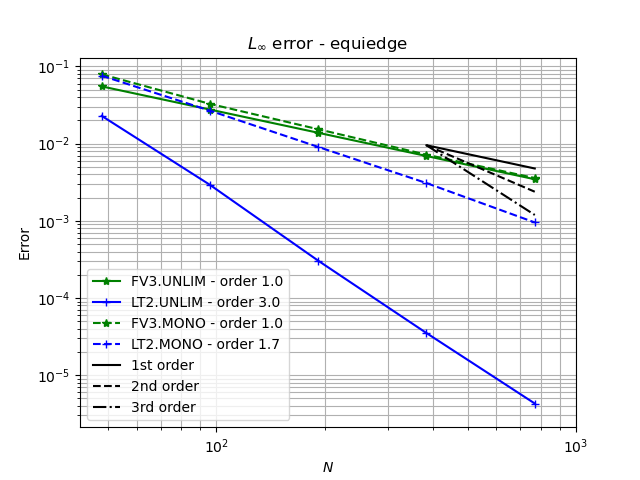
\includegraphics[width=1.1\linewidth]{linferror_tc-6_alpha0.equiedge}
		\caption{Equi-edge grid\label{divnair-equiedge-linf}}
	\end{subfigure}
	\caption{
		$L_{\infty}$ error convergence for the tracer concentration $\phi$ in the transport model using the two Gaussian hills  as the initial condition and  the divergent deformational wind on equiangular  (a)
		and equi-edge (b) grids  after 12 days.
		Blue lines indicate the use of the LT2 scheme, while green lines represent the FV3 scheme.
		Solid lines represent the results with the unlimited PPM (UNLIM) scheme, whereas dashed lines represent the results with the monotonic PPM (MONO).
		\label{divnair-linf}}
\end{figure}


\begin{figure}[!htb]
	\centering
	\begin{subfigure}{0.45\textwidth}
		\centering
		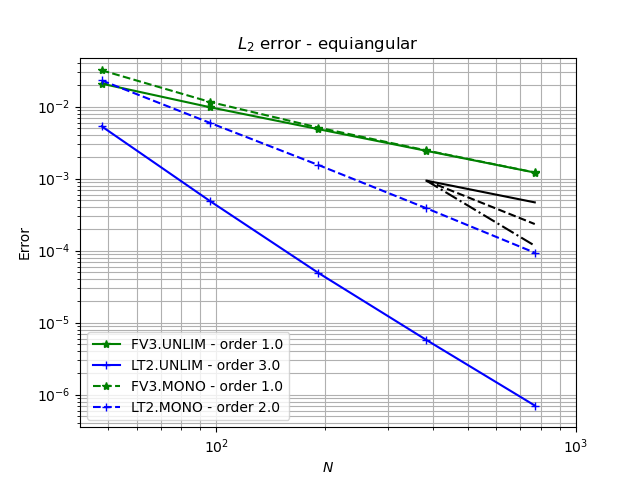
\includegraphics[width=1.1\linewidth]{l2error_tc-6_alpha0.equiangular}
		\caption{Equiangular grid\label{divnair-equiangular-2}}
	\end{subfigure}
	\begin{subfigure}{0.45\textwidth}
	\centering
	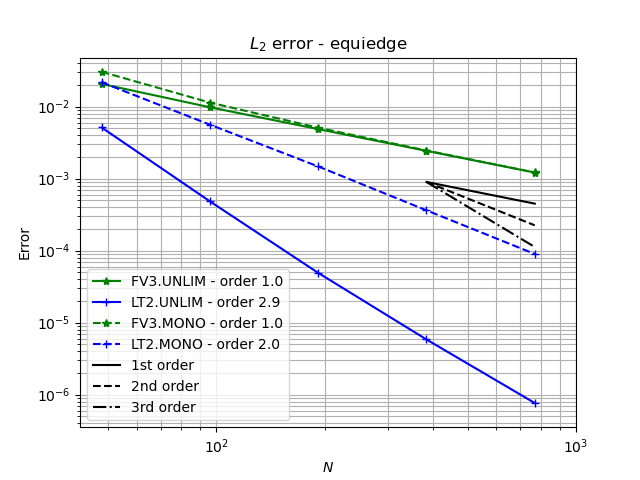
\includegraphics[width=1.1\linewidth]{l2error_tc-6_alpha0.equiedge}
  	\caption{Equi-edge grid\label{divnair-equiedge-l2}}
    \end{subfigure}
	\caption{As Figure \ref{divnair-linf} but using $L_2$ norm.
		\label{divnair-l2}}
\end{figure}

Figures \ref{divnair-linf} and \ref{divnair-l2} show the error convergence in $L_{\infty}$ and $L_{2}$ norms for the tracer concentration $\phi$.
These figures highlight a major significant distinction between LT2 and FV3 schemes, unlike the previous tests.
It is clear that FV3 with the unlimited PPM achieves only first-order accuracy, whereas LT2 with the unlimited PPM achieves third-order accuracy, 
surpassing second-order the expectation, for both equi-edge and the equiangular grids and error norms.
For the monotonic scheme, LT2 demonstrates second-order accuracy in the $L_2$ norm, while FV3 is only first-order.
LT2 with the monotonic scheme, exhibits smaller errors in the $L_{\infty}$ norm compared to the FV3 scheme for all grids.
This discrepancy arises because the FV3 splitting is designed for divergence-free flows, while LT2 is designed to be second-order regardless of the flow characteristics.

%%%%%%%%%%%%%%%%%%%%%%%%%%%%%%%%%%%%%%%%%%%%%%%%%%%%%%%%%%%%%%
\section{Concluding remarks}
\label{conclusion}
\textcolor{red}{This work has revisited the FV3 transport scheme in all its details}. This thorough examination has allowed for proposed modifications to improve the accuracy of the FV3 advection scheme, leading to a proposed scheme named LT2.

The FV3 transport scheme relies on applying 1D finite-volume fluxes, namely the PPM, using a direction-splitting strategy.
\textcolor{red}{The proposed modifications to the 1D scheme aim to allow a more accurate treatment in handling metric terms and computing the departure points.}
Furthermore, the FV3 scheme combines the 1D fluxes in such a way that the splitting error for a constant scalar field and divergence-free wind is eliminated.
In contrast, the LT2 scheme does not have this property but introduces a second-order error in this case.

\textcolor{red}{To compare both schemes, this paper has considered a transport model on the sphere, where it is needed to solve two conservative transport equations: one for the tracer concentration and another for the fluid density. 
Subsequently, numerical simulations were conducted with both schemes.}

The LT2 scheme showed to  have slightly smaller errors than the FV3 scheme for divergence-free winds.
Both schemes are second-order when no limiter is employed and the wind is divergence-free.
The major difference between FV3 and LT2 is when the wind is not divergence-free.
In this case, FV3 is only first order, while LT2 is second-order. Even with a limiter, LT2 is much more accurate than FV3 in this case, \textcolor{red}{specially in the $L_2$ norm.}
This was demonstrated consistently throughout the simulations.
Therefore, the major conclusion here is that the LT2 scheme is more accurate regardless of whether the wind is divergence-free or not, while FV3 is only accurate for divergence-free winds.

%Furthermore, during the advection a Gaussian hill through a rotated zonal wind, both FV3 and LT2 schemes exhibited small spikes in errors whenever the Gaussian hill passed over a corner. 
%Overall, the LT2 scheme showed slightly smaller errors in this test.
%Additionally, \textcolor{red}{it was} observed that the equi-edge grid generally exhibited smaller errors compared to the equiangular grid for all simulations, with the LT2 scheme demonstrating good results in both grids.



\textcolor{red}{
Although this paper has considered the transport model, the ultimate goal is to use the LT2 scheme within the full three-dimensional non-hydrostatic solver. 
In particular, the LT2 scheme may be used to compute the fluid depth and the absolute vorticity fluxes in the shallow-water equations that are solved in the three-dimensional non-hydrostatic solver along the Lagrangian surfaces \cite{lin:2004}.}

\textcolor{red}{
It is anticipated that shallow-water numerical experiments were also conducted using both the FV3 and LT2 schemes, along with the test cases from \cite{will:1992} and \cite{galewsky:2004}. It was observed that the LT2 scheme did not deteriorate the accuracy of the shallow-water solver. 
Both schemes showed very similar results for these shallow-water tests.
This is expected, as most of the shallow-water tests available on the literature have small or no wind divergence.
We are currently working on developing a test for the shallow-water equations where divergence plays a key role in the solution dynamics to test the LT2 and FV3 schemes in this case.
In this scenario, it is expected that the LT2 scheme should introduce a more accurate solution.}

\textcolor{red}{
Horizontal wind divergence plays a pivotal role in many phenomena on the atmosphere such as in tropical cyclones, hurricanes and in the Intertropical Convergence Zone \cite{holton:2012}.
For example, hurricanes are fueled by strong horizontal wind convergence at the Earth’s surface, with strong horizontal wind divergence occurring at high altitudes.
Therefore, we expect that the LT2 scheme has the potential to improve the forecast of these phenomena where wind divergence is present.
For example, LT2 scheme may be used to conduct a study based on \cite{gao:2021}, where the impact of using different 1D PPM schemes of FV3 on hurricane intensity prediction is investigated. 
This study highlights how modifying the advection scheme may improve hurricane intensity prediction and affect the eyewall convection location.
}



\section*{CRediT authorship contribution statement}
\textcolor{red}{To be written.}

\section*{Declaration of competing interest}
The authors declare that they have no known competing financial interests or personal relationships that could have appeared to influence the work reported in this paper.

\section*{Data availability}
The source code used in this work is available at \url{https://github.com/luanfs/FV3_container}.
This code was executed using Docker, utilizing the containerized
version of the SHiELD model developed by \cite{cheng:2022}.

\section*{Acknowledgments}
We acknowledge the financial support provided by the São Paulo Research Foundation (FAPESP) under the grants 2020/10280-4 and 2021/06176-0.



\appendix
\section{Metric term relations}
\label{metric_terms}
A straightforward computation using Equation \eqref{gamma_1} shows that the derivatives of the mappings $\Gamma_p$ are explicitly given by:
\begin{align}
	\label{dgamma_1}
	d{\Gamma}_{1}(X,Y) &= \frac{R}{{(1 + X^2 + Y^2)}^{3/2}}
	\begin{bmatrix}
		-X & -Y \\
		1+Y^2  & -XY \\
		-XY  & 1+X^2
	\end{bmatrix},
\end{align}
and similar formula holds for the other values of $p$.
Thus, it follows that the metric tensor of $\Gamma_p$ is explicitly given by
\begin{align}
	\label{gamma_tensor_explicity}
	G_{{\Gamma}}(X,Y) = 
	\frac{R^2}{(1 + X^2 + Y^2)^2}
	\begin{bmatrix}
		1+ X^2 &  -XY \\
		-XY & 1 + Y^2
	\end{bmatrix},
\end{align}
and the metric term of $\Gamma_p$ is given by:
\begin{equation}
	\label{mt_gamma_explicity}
	\sqrt{\mathfrak{g}_{{\Gamma}}}(X,Y) = \frac{R^2}{(1+X^2+Y^2)^{3/2}}.
\end{equation}
It follows from the chain rule in Equation \eqref{psi-def} that:
\begin{equation}
	\label{dpsi}
	d {\Psi}_p(x,y) = d {\Gamma}_p\big(\beta(x),\beta(y)\big)\cdot\text{diag}\big(\beta'(x),\beta'(y)\big),
\end{equation}
where $\text{diag}(\beta'(x),\beta'(y))$ is a diagonal $2\times 2$ matrix with diagonal entries given by $\beta'(x)$ and $\beta'(y)$.
The tangent vector basis $\{{\partial_x  {\Psi}_p},  {\partial_y  {\Psi}_p}\}$ satisfies:
\begin{align}
	\label{dx_psi}
	{\partial_x  {\Psi}_p}(x,y) = \beta'(x) \cdot {\partial_X 
		{\Gamma}_p}\big(\beta(x),\beta(y)\big),\\
	\label{dy_psi}
	{\partial_y  {\Psi}_p}(x,y) = \beta'(y) \cdot {\partial_Y  {\Gamma}_p}\big(\beta(x),\beta(y)\big).
\end{align}
Finally, the metric term $\sqrt{\mathfrak{g}_{\Psi}}$ is expressed in terms of $\sqrt{\mathfrak{g}}_{\Gamma}$ as
\begin{align}
	\sqrt{\mathfrak{g}_{\Psi}}(x,y) &= \beta'(x)\beta'(y)\sqrt{\mathfrak{g}}_{\Gamma}\big(\beta(x),\beta(y)\big)\\
	&= \beta'(x)\beta'(y)\frac{R^2}{\big(1+\beta(x)^2+\beta(y)^2\big)^{3/2}}.
\end{align}

\section{Relations between wind representation on the cubed-sphere and on latitude-longitude coordinates}
\label{ap-wind}
We consider the latitude-longitude mapping 
${\Pi}: [-\pi,\pi] \times [-\frac{\pi}{2},\frac{\pi}{2}] \to \mathbb{S}^2_R$, 
${\Pi} = ({\Pi}_1,{\Pi}_2,{\Pi}_3)$, given by:
\begin{align}
	\label{ll2sph}
	{\Pi}_1(\lambda,\theta) &= R\cos \theta \cos \lambda,\\
	{\Pi}_2(\lambda,\theta) &= R\cos \theta \sin \lambda,\\
	{\Pi}_3(\lambda,\theta) &= R\sin \theta.
\end{align}
Using this mapping,  the unit tangent vectors may be computed as:
\begin{equation}
	\label{latlon_tg_vectors}
	\boldsymbol{e}_{\lambda}(\lambda,\theta) = 
	\begin{bmatrix}
		-\sin \lambda \\
		\cos \lambda \\
		0
	\end{bmatrix}, \quad
	\boldsymbol{e}_{\theta}(\lambda,\theta) =
	\begin{bmatrix}
		-\sin \theta \cos \lambda \\
		-\sin \theta \sin \lambda \\
		\cos \theta
	\end{bmatrix}.
\end{equation}
A tangent vector field $\boldsymbol{u}$ on the sphere may be then written in terms of $\boldsymbol{e}_{\theta}$ and $\boldsymbol{e}_{\lambda}$ as:
\begin{equation}
	\label{latlon-wind}
	\boldsymbol{u}(\lambda, \theta) = 
	u_{\lambda} (\lambda, \theta) \boldsymbol{e}_{\lambda} (\lambda, \theta) + 
	v_{\theta} (\lambda, \theta) \boldsymbol{e}_{\theta} (\lambda, \theta), 
\end{equation}
where $u_{\lambda}$ is the zonal component and $v_{\theta}$ is the meridional component.
The latitude-longitude representation is related with the normalized contravariant representation (Equation \eqref{norm-contravariant-wind})  by the expression:
\begin{equation}
	\label{ll-to-normcontravariant}
	\begin{bmatrix}
		u_\lambda (\lambda, \theta) \\
		v_\theta (\lambda, \theta) 
	\end{bmatrix}
	=
	\begin{bmatrix}
		\langle 	\boldsymbol{e}_x, \boldsymbol{e}_\lambda \rangle 
		& \langle 	\boldsymbol{e}_y, \boldsymbol{e}_\lambda \rangle \\
		\langle 	\boldsymbol{e}_x, \boldsymbol{e}_\theta \rangle 
		& \langle 	\boldsymbol{e}_y, \boldsymbol{e}_\theta \rangle \\
	\end{bmatrix}
	\begin{bmatrix}
		{u}(x,y,p) \\
		{v}(x,y,p)
	\end{bmatrix},
\end{equation}
which holds since $\boldsymbol{e}_{\lambda}$ and $\boldsymbol{e}_{\theta}$
are orthogonal. This formula is just a basis conversion.
%The covariant components $(\mathfrak{U},\mathfrak{V})$ are given by:
%\begin{align}
%	\label{covariant-u}
%	\mathfrak{U}(x,y) = \langle \boldsymbol{u}(x,y) , 	\partial_x\boldsymbol{\Psi}_p(x,y)  \rangle, \quad
%	\mathfrak{V}(x,y) = \langle \boldsymbol{u}(x,y) , 	\partial_y\boldsymbol{\Psi}_p(x,y)  \rangle.
%\end{align}
%Like the contravariant component, FV3 works with the normalized covariant wind $({U},{V})$ given by:
%\begin{align}
%	\label{norm-covariant-u}
%	{U}(x,y) = \langle \boldsymbol{u}(x,y) , \boldsymbol{e}_y(x,y)  \rangle, \quad
%	{V}(x,y) = \langle \boldsymbol{u}(x,y) , \boldsymbol{e}_y(x,y)  \rangle.
%\end{align}
%It is easy to see that:
%\begin{equation}
%	\label{covari-uv}
%	{U}(x,y)  = \frac{\mathfrak{U}(x,y)}{\|\partial_x\boldsymbol{\Psi}_p(x,y)\|}, \quad
%	{V}(x,y)  = \frac{\mathfrak{V}(x,y)}{\|\partial_y\boldsymbol{\Psi}_p(x,y)\|}.
%\end{equation}
%Replacing Equation \eqref{norm-contravariant-wind} in 
%Equation \eqref{norm-covariant-u} we obtain
%the relation between normalized covariant components in terms of the
%normalized contravariant terms:
%\begin{equation}
%	\label{norm-contravariant-to-covariant}
%	\begin{bmatrix}
%		{U}(x,y) \\
%		{V}(x,y)
%	\end{bmatrix}
%	=
%	\begin{bmatrix}
%		1 
%		& \langle 	\boldsymbol{e}_x, \boldsymbol{e}_y \rangle \\
%		\langle 	\boldsymbol{e}_x, \boldsymbol{e}_y \rangle 
%		& 1\\
%	\end{bmatrix}
%	\begin{bmatrix}
%		{u} (x,y) \\
%		{v} (x,y) 
%	\end{bmatrix}.
%\end{equation}
%Recall that
%\begin{equation}
%	\langle 	\boldsymbol{e}_x, \boldsymbol{e}_y \rangle(x,y) = \cos \alpha(x,y),
%\end{equation}
%where $\alpha(x,y)$ is the angle between and 	%$\boldsymbol{e}_x$, $\boldsymbol{e}_y$, which
%is the formula implemented in FV3 following \cite{putman:2007}.

%\newpage
\section{Relation between time-averaged fluxes and departure points}
\label{app-flux}
In the following theorem, it is proven how the time-averaged flux is related to a spatial integral over a interval depending on departure points.
\newtheorem{theorem}{Theorem}
\begin{theorem}
\label{flux-theorem}
Assume that $q$ and $\mathfrak{u}$ are $\mathcal{C}^1$ functions and that 
$q$ satisfies Equation \eqref{1d-avd-eq}, then:
\begin{equation}
	\label{chp2-sec-flux:approx1}
	\int_{t^n}^{t^{n+1}} (\mathfrak{u}\sqrt{\mathfrak{g}}q)(x_{i+\frac{1}{2}},s) \,ds = 
	\int^{x_{i+\frac{1}{2}}}_{ x_{i+\frac{1}{2}}^d(t^n,t^{n+1})} (\sqrt{\mathfrak{g}}q)(x,t^n)\,dx.
\end{equation}
\end{theorem}


\begin{proof}
\textcolor{red}{
To start with, the variable $\varphi = \sqrt{\mathfrak{g}}q$ is introduced to simplify the notation.
Let us consider the mapping $s\in[t^n,t^{n+1}] \to  x_{i+\frac{1}{2}}^d(t^n,s)$. 
Integrating $\varphi$ at time $t^n$ over all the range of $x_{i+\frac{1}{2}}^d(t^n,s)$ for $s\in[t^n,t^{n+1}]$ yields:
\begin{equation}
	\label{depint_1}
	\int_{x_{i+\frac{1}{2}}^d(t^n,t^{n+1})}^{x_{i+\frac{1}{2}}}   
	\varphi(x,t^n)\,dx 
	= -\int_{t^n}^{t^{n+1}}  \varphi\big( x_{i+\frac{1}{2}}^d(t^n,s),t^n\big){\partial_s}{ x_{i+\frac{1}{2}}^d} (t^n,s)\,ds,
\end{equation}
which follows from the variable change integration formula, recalling that ${ x_{i+\frac{1}{2}}^d(t^n,t^{n}) = x_{i+\frac{1}{2}}}$. 
Hence, it suffices to prove that:
\begin{equation}
	\label{phi-u}
	\varphi\big( x_{i+\frac{1}{2}}^d(t^n,s),t^n\big){\partial_s}{ x_{i+\frac{1}{2}}^d} (t^n,s) = -(\mathfrak{u}\varphi)(x_{i+\frac{1}{2}},s).
\end{equation}
Firstly, ${\partial_s x_{i+\frac{1}{2}}^d}(t,s)$ is computed using the Leibniz rule for integration in Equation \eqref{dp-integral}, which leads to
\begin{align}
	\begin{split}
		\label{dxds}
		{\partial_s x_{i+\frac{1}{2}}^d} (t,s) &= - \bigg(\mathfrak{u}(x_{i+\frac{1}{2}},s) + 
		\int_{t}^{s} {\partial_s\mathfrak{u}}\big( x_{i+\frac{1}{2}}^d(\tau,s),\tau\big) \,d\tau \bigg)\\
		&=- \mathfrak{u}(x_{i+\frac{1}{2}},s) -
		\int_{t}^{s} {\partial_x}{\mathfrak{u}}\big( x_{i+\frac{1}{2}}^d(\tau, s),\tau\big) 
		{\partial_s  x_{i+\frac{1}{2}}^d}(\tau, s)\,d\tau.
	\end{split}
\end{align}
Taking the derivative with respect to $t$ of Equation \eqref{dxds}, one gets:
\begin{equation}
	\label{dxds_2}
	{\partial_t }{\partial_s  x_{i+\frac{1}{2}}^d}
	(t,s) = {\partial_x}{\mathfrak{u}}\big(x_{i+\frac{1}{2}}^d(t, s), t\big) 
	{\partial _s} x_{i+\frac{1}{2}}^d (t, s).
\end{equation}
One check upon inspection that the trajectory $x_{i+\frac{1}{2}}^d$ that solves Equations \eqref{dxds} and \eqref{dxds_2} is given by:
\begin{equation}
	\label{xs_int}
	{\partial_s  x_{i+\frac{1}{2}}^d}(t,s) = -
	\exp{\bigg(\int_{t}^{s} {\partial_x}{\mathfrak{u}}\big( x_{i+\frac{1}{2}}^d(\tau,s),\tau\big)  \,d\tau \bigg)}
	\mathfrak{u}(x_{i+\frac{1}{2}},s).
\end{equation}
Secondly, to obtain $\varphi\big(x_{i+\frac{1}{2}}^d(t^n,s),t^n\big)$, we compute $\varphi$ along the trajectory given by $x_{i+\frac{1}{2}}^d(t,s)$, and then take its time derivative:
\begin{align}
	\label{dqdt}
	\begin{split}
		\frac{d}{dt}\varphi\big( x_{i+\frac{1}{2}}^d(t,s),t\big) &= 
		{\partial_t}\varphi\big( x_{i+\frac{1}{2}}^d(t,s),t\big)+
		(\mathfrak{u}{\partial_x } 
		\varphi)\big(x_{i+\frac{1}{2}}^d(t,s),t\big) \\
		&= -{\partial_x}{\mathfrak{u}}\big( x_{i+\frac{1}{2}}^d(t,s),t\big) \varphi \big(x_{i+\frac{1}{2}}^d(t,s),t\big),
	\end{split}
\end{align}
where we used that $\varphi$ satisfies Equation \eqref{1d-avd-eq} and that $x_{i+\frac{1}{2}}^d(t,s)$
solves Equation \eqref{1d-dp-equation}.
One check upon inspection again that $\varphi$ that solves Equation \eqref{dqdt} is given by:
\begin{equation}
	\label{q_int}
	\varphi\big( x_{i+\frac{1}{2}}^d(t,s),t\big) = 
	\exp{\bigg(-\int_{t}^{s} {\partial_x}{\mathfrak{u}}\big( x_{i+\frac{1}{2}}^d(\tau,s),\tau\big)  \,d\tau \bigg)}
	\varphi(x_{i+\frac{1}{2}},s).
\end{equation}
Equation \eqref{phi-u} can be obtained by multiplying Equation \eqref{xs_int} by Equation \eqref{q_int} at $t=t^n$, which concludes the proof.}
\end{proof}

\end{linenumbers}
%\newpage
  \bibliographystyle{elsarticle-num} 
  \bibliography{references}

%% else use the following coding to input the bibitems directly in the
%% TeX file.

%% Refer following link for more details about bibliography and citations.
%% https://en.wikibooks.org/wiki/LaTeX/Bibliography_Management

%\begin{thebibliography}{00}

%% For numbered reference style
%% \bibitem{label}
%% Text of bibliographic item

%bibitem{lamport94}
%  Leslie Lamport,
%  \textit{\LaTeX: a document preparation system},
%  Addison Wesley, Massachusetts,
%  2nd edition,
%  1994.

%\end{thebibliography}
\end{document}

\endinput
%%
%% End of file `elsarticle-template-num.tex'.
